    Наиболее простым видом столкновительно-индуцированных спектров являются трансляционные спектры, порождаемые смесью двух благородных газов при низком давлении, где доминируют бинарные столкновения. При более высоких давлениях будут случаться столкновения с участием трех и более атомов, которые будут видоизменять форму спектра поглощения. На рис. \ref{pic-two-atom-experiment} приведены примеры экспериментальных столкновительно-индуцированных спектров поглощения в дальней ИК области систем He$-$Ar, Ne$-$Ar и Ar$-$Kr \cite{frommhold}. Было экспериментально подтверждено, что интенсивность поглощения линейно зависит от произведения плотностей газов $\rho_1 \rho_2$, что говорит о том, что спектр порождается парами разных атомов. Отклонение от линейной зависимости будет говорить о том, что при данных концентрациях существенный вклад вносят многочастичные столкновения. Спектры, изображенные на рис \ref{pic-two-atom-experiment}, сняты при разных концентрациях от 60 амага (He$-$Ar) до 200 амага (Ar$-$Kr).  

\begin{figure}[H]
    \centering
    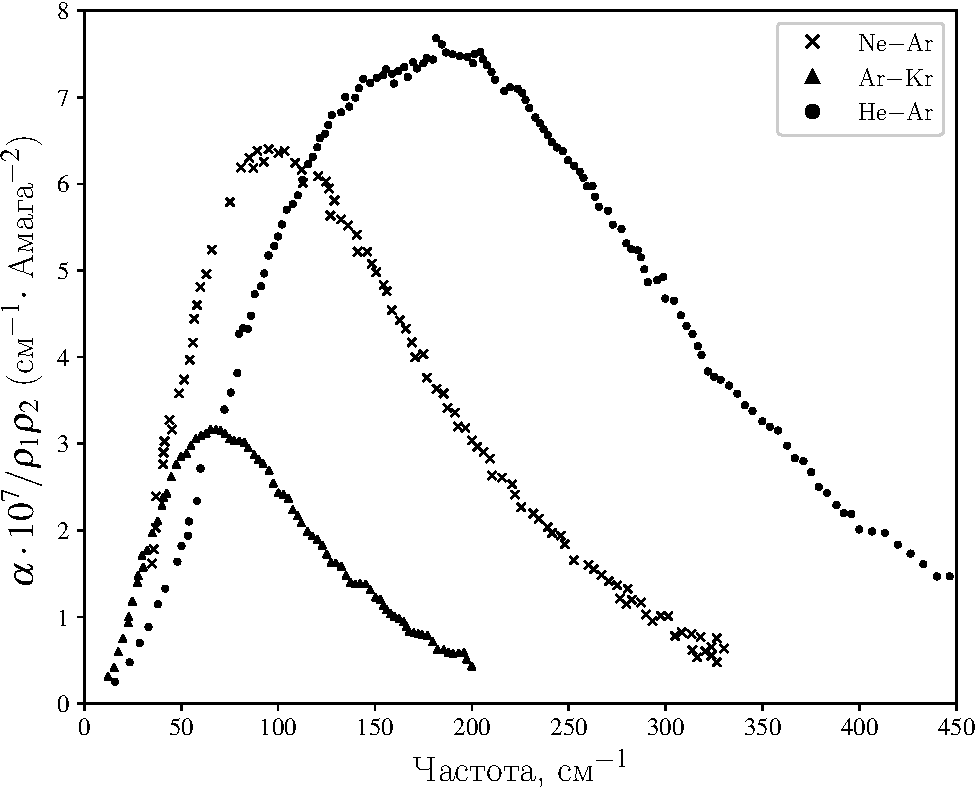
\includegraphics[width=0.7\linewidth]{./pictures/twoatom_experiment/experiment_diatom_spectra-crop.pdf}
    \label{pic-two-atom-experiment}
    \caption{Экспериментальные спектры бинарного поглощения систем гелий$-$аргон, неон$-$аргон и аргон$-$криптон при комнатной температуре \cite{frommhold}}
\end{figure}

В работе \cite{kranendonk1973} авторы разрабатывают формализм расчета столкновительно-индуцированного спектра в приближении бинарных столкновений. Авторы рассматривают систему, состояющую из молекулы $H_2$, возмущенной атомами $Ar$. Вращательное движение молекулы $H_2$ исключено из рассмотрения -- обе сталкивающихся молекулы рассматриваются как безструктурные сферически-симметричные частицы. \par
    Спектральная функция, определяющая профиль спектра поглощения, связана с функцией автокорреляции суммарного дипольного момента системы преобразованием Фурье
\begin{gather}
    J(\omega) = \intty \mean{ \bs{\mu}(0) \bs{\mu}(t) } e^{i \omega t} dt. \label{twoatom-spectral-function}
\end{gather} 
В приближении бинарных столкновений корреляционная функция суммарного дипольного момента становится 
\begin{gather}
    \mean{ \bs{\mu}(0) \bs{\mu}(t) } = N \mean{ \bs{\mu}_1(0) \bs{\mu}_1(t) },
\end{gather} 
%
где через $\bs{\mu_1}(t)$ обозначен дипольный момент индуцированный квадрупольным полем молекулы $H_2$ на атоме $Ar$, а $N$ -- количество рассматриваемых пар. Приведенную массу системы обозначают через $\mu$; вектор, соединяющий центр масс молекулы $H_2$ атомом $Ar$ -- через $\mathbf{R}$; потенциал взаимодействия -- через $V(R)$ $[$как уже говорилось, вращательное движение молекулы водорода не рассматривается, поэтому потенциал зависит только от расстояния между центрами масс $R$$]$. Автокорреляционную функцию дипольного момента приводят к виду 
\begin{gather}
    C(\tau) = \frac{N}{V} \lb \frac{\mu}{2 \pi k T} \rb^{3/2} \iint \bs{\mu}_1(\mathbf{R}) \cdot \bs{\mu}_1(\mathbf{R}(\tau)) \exp \lb -\frac{\mu \dot{\mf{R}}^2}{2 k T} \rb g_0(R) \, d \mathbf{R} \, d \dot{\mathbf{R}}, \label{kranendonk-correlation-function}
\end{gather}
%
где $\mathbf{R}(\tau)$ -- значение $\mathbf{R}$, вычисленное в момент времени $\tau$ путем расчета классической траектории, начальными условиями для которой взяты $\mf{R}$ и $\dot{\mf{R}}$, и $g_0(R)$ -- парная функция распределения (вероятность того, что между атомами расстояние $R$)
\begin{gather}
    g_0(R) = \exp \lb -\frac{V(R)}{kT} \rb.
\end{gather}

Выражение \eqref{kranendonk-correlation-function} неудобно для численного расчета, т.к. в нем имеется $R(\tau)$ для произвольного момента времени $\tau$. Для более эффективной вычислительной схемы предлагается переписать интегральное выражение \eqref{kranendonk-correlation-function} как интеграл по полным столкновительным траекториям. При этом будут рассматриваться только траектории рассеяния. В лабораторной системе отсчета энергия система может быть записана в виде
\begin{gather}
    E = \frac{1}{2} \mu \dot{\mf{R}}^2 + V(R).
\end{gather}
Траекторию рассеяния, которая имеет в момент времени $t$ радиус-вектор $\mf{R}$ и скорость $\dot{\mf{R}}$, может быть однозначно определена относительной скоростью $\mf{g}$ в момент времени $t = -\infty$, прицельным параметром $b$, углом, определяющим ориентацию плоскости столковения $\varepsilon$, и моментом времени $t_0$, в которое произошло столкновение. Применяя теорему Лиувилля
\begin{gather}
    d \mf{R} \, d\dot{\mf{R}} = g d(t - t_0) b db \, d\varepsilon \, d\mf{g},
\end{gather}
%
выражение \eqref{kranendonk-correlation-function} преобразуют к виду
\begin{gather}
    C(\tau) = \frac{N}{V} \lb \frac{\mu}{2 \pi k T} \rb^{3/2} \idotsint \bs{\mu}_1(t) \cdot \bs{\mu}_1(t + \tau) \, g \exp \lb - \frac{\mu \mf{g}^2}{2 k T} \rb b \, db \, d\varepsilon \, d \mf{g}. \label{correlation-function-kranendonk}
\end{gather}

Корреляцией двух функций $f$ и $g$, определенных на комплексной плоскости $\mathbb{C}$, называют функцию, определенную следующим интегралом
\begin{gather}
    C(\tau) = \intty f^{*}(t) g(\tau + t) dt,
\end{gather}
% 
где $*$ обозначает комплексное сопряжение. Обозначим через $F(\omega)$, $G(\omega)$ Фурье-образы функций $f(t)$, $g(t)$. Перепишем выражение для корреляции, представив функции через обратное преобразование Фурье от $F(\omega)$, $G(\omega)$, соответственно.
\begin{gather}
    C(\tau) = \intty \lsq \, \intty F^{*}(\omega) e^{-i \omega t} \frac{d \omega}{2 \pi} \rsq \lsq \, \intty G(\omega^\prime) e^{i \omega^\prime (\tau + t)} \frac{d\omega^\prime}{2 \pi} \rsq
\end{gather}

Осуществляя перестановку внутри интегрального выражения, приходим к следующему выражению 
\begin{gather}
    C(\tau) = \frac{1}{2\pi} \intty \intty F^*(\omega) G(\omega^\prime) e^{i \omega^\prime \tau} \lsq \, \intty e^{i (\omega^\prime - \omega) t} \frac{dt}{2 \pi} \rsq d\omega d\omega^\prime = \notag \\
    = \frac{1}{2\pi} \intty \inty F^*(\omega) G(\omega^\prime) e^{i \omega^\prime \tau} \delta \lb \omega^\prime - \omega \rb d\omega d\omega^\prime = \hat{F}^{-1} \Big[ F^*(\omega) G(\omega) \Big],
\end{gather}
%
где через $\hat{F}$ обозначен оператор преобразования Фурье. Если рассмотреть эту цепочку преобразований для автокорреляционной функции действительной функции $f(t)$, то приходим к теореме Винера-Хинчина \cite{frommhold}
\begin{gather}
    \hat{F} \Big[ C(\tau) \Big] = \Big\vert \hat{F}\Big[ f(t) \Big] \Big\vert^2. 
\end{gather}

Автокорреляционная функция дипольного момента распадается на сумму автокорреляционных функций его компонент
\begin{gather}
    C(\tau) = \intty \bs{\mu}_1(t) \bs{\mu}_1(t + \tau) dt = \sum_{\alpha = x, y, z} \intty \mu_1^\alpha(t) \mu_1^\alpha(t + \tau) dt = C_x(\tau) + C_y(\tau) + C_z(\tau).
\end{gather}

Следовательно, преобразование Фурье от автококорреляционной функции дипольного момента представляет собой сумму квадратов преобразований Фурье от компонент дипольного момента
\begin{gather}
    \hat{F}\Big[ C(\tau) \Big] = \sum_{\alpha = x,y,z} \hat{F} \Big[ C_\alpha(\tau) \Big] = \sum_{\alpha=x,y,z} \Bigg\vert \intty \mu_1^\alpha(t) e^{-i\omega t} dt \Bigg\vert^2,
\end{gather}
% 
что для краткости обозначают 
\begin{gather}
    \hat{F} \Big[ C(\tau) \Big] = \Bigg\vert \intty \bs{\mu}_1(t) e^{-i\omega t} dt \Bigg\vert^2. \label{correlation-theorem}
\end{gather}

Итак, преобразование Фурье от автокорреляционной функции \eqref{correlation-function-kranendonk} дает спектральную функцию  
\begin{gather}
    J(\omega) = \frac{N}{V} \lb \frac{\mu}{2 \pi k T} \rb^{3/2} \idotsint \Bigg\vert \intty \bs{\mu}_1(t) e^{-i \omega t} dt \Bigg\vert^2 \, \exp \lb -\frac{\mu g^2}{2 k T} \rb b \, db \, d \varepsilon \, 4 \pi g^3 dg.
\end{gather}

\section{Cистемы координат для описания движения двух атомов}

Рассмотрим движение двух атомов с массами $m_1$, $m_2$ с радиус - векторами $\mf{r}_1$, $\mf{r}_2$ в поле межатомного потенциала $U(\vert \mf{r}_1 - \mf{r}_2 \vert)$. Задача о движении двух взаимодействующих атомов сводится к задаче о движении виртуальной частицы с приведенной массой $\mu$,  равной 
\begin{gather}
    \mu = \frac{m_1 m_2}{m_1 + m_2}, 
\end{gather}
%
в заданном потенциальном поле $U$ \cite{landau-volume1}. Для описания движения виртуальной частицы введем несколько систем координат. Системой I будем называть декартову систему координат -- положение частицы задается вектором $\mf{r} = \mf{r}_1 - \mf{r}_2$. В этой системе координат лагранжиан и гамильтониан системы записываются как 
\begin{gather}
    \mL_\text{cartesian} = \frac{\mu \dot{\mf{r}}^2}{2} - U( \vert \mf{r} \vert ), \label{two-atom-cartesian-lagrangian} \\
    \mH_\text{cartesian} = \frac{\mf{p}^2}{2\mu} + U( \vert \mf{r} \vert ), \label{two-atom-cartesian-hamiltonian}
\end{gather}
%
где вектор импульса $\mf{p}$ равен
\begin{gather}
    \mf{p} = \frac{\partial \mL_\text{cartesian}}{\partial \dot{\mf{r}}} = \mu \, \dot{\mf{r}}. \label{two-atom-cartesian-momenta}
\end{gather}

Вектор $\mf{r}$ можно представить в сферической системе координат -- длину вектора обозначим через $r$, зенитный и азимутальный углы через $\theta$ и $\varphi$, соответственно ($\theta \in [0, \pi], \phi \in [0, 2 \pi]$. Будем называть эту координатную систему системой II. Лагранжиан и гамильтониан в ней записываются как
\begin{gather}
    \mL_\text{spherical} = \frac{1}{2} \mu \dot{r}^2 + \frac{1}{2} \mu r^2 \dot{\theta}^2 + \frac{1}{2} \mu r^2 \dot{\varphi}^2 \sin^2 \theta - U(r),  \label{two-atom-spherical-lagrangian} \\
    \mH_\text{spherical} = \frac{p_r^2}{2 \mu} + \frac{p_\theta^2}{2 \mu r^2} + \frac{p_\varphi^2}{2 \mu r^2 \sin^2 \theta} + U(r), \label{two-atom-spherical-hamiltonian}
\end{gather}
%
где обобщенные импульсы $p_r$, $p_\theta$, $p_\varphi$ связаны с обобщенными скоростями соотношениями
\begin{gather}
    p_r = \frac{\partial \mL_\text{spherical}}{\partial \dot{r}} = \mu \dot{r}, \quad \dot{r} = \frac{p_r}{mu} \label{two-atom-spherical-momenta1} \\
    p_\theta = \frac{\partial \mL_\text{spherical}}{\partial \dot{\theta}} = \mu r^2 \dot{\theta}, \quad \dot{\theta} = \frac{p_\theta}{\mu r^2} \label{two-atom-spherical-momenta2} \\
    p_\varphi = \frac{\partial \mL_\text{spherical}}{\partial \dot{\varphi}} = \mu r^2 \dot{\varphi} \sin^2 \theta \quad \dot{\phi} = \frac{p_\varphi}{\mu r^2 \sin^2 \theta} \label{two-atom-spherical-momenta3}.
\end{gather}

Декартовы координаты виртуальной частицы связаны со сферическими координатами следующими соотношениями
\begin{gather}
    \lc
    \begin{aligned}
        x &= r \cos \varphi \sin \theta \\
        y &= r \sin \varphi \sin \theta \\
        z &= r \cos \theta
    \end{aligned}
    \right. \label{two-atom-spherical-coordinates}
\end{gather}

Рассмотрим, как связаны декартовы импульсы $\mf{p}$ с импульсами $p_r$, $p_\theta$, $p_\phi$, сопряженными сферическим координатам. Для этого продифференцируем соотношения \eqref{two-atom-spherical-coordinates} по времени и умножим обе части на приведенную массу $\mu$, получив в левой части компоненты вектора $\mf{p}$ согласно \eqref{two-atom-cartesian-momenta}, а в правой части подставим выражения обобщенных скоростей $\dot{r}$, $\dot{\theta}$, $\dot{\varphi}$ через соответствующие импульсы \eqref{two-atom-spherical-momenta1}, \eqref{two-atom-spherical-momenta2}, \eqref{two-atom-spherical-momenta3}
\begin{gather}
    \lc 
    \begin{aligned}
        p_x &= p_r \cos \varphi \sin \theta + \frac{p_\theta}{r} \cos \varphi \cos \theta - \frac{p_\varphi}{r} \frac{\sin \varphi}{\sin \theta} \\ 
        p_y &= p_r \sin \varphi \sin \theta + \frac{p_\theta}{r} \sin \varphi \cos \theta + \frac{p_\varphi}{r} \frac{\cos \varphi}{\sin \theta} \\ 
        p_z &= p_r \cos \theta - \frac{p_\theta}{r} \sin \theta 
    \end{aligned}
    \right. \label{two-atom-cartesian-spherical-momenta}
\end{gather}

Разрешая линейные соотношения \eqref{two-atom-cartesian-spherical-momenta} относительно импульсов $p_r$, $p_\theta$, $p_\varphi$, находим соотношения, выражающие обратную связь импульсов.
\begin{gather}
    \lc
    \begin{aligned}
        p_r &= r \lb p_x \cos \varphi \sin \theta + p_y \sin \varphi \sin \theta + p_z \cos \theta \rb\\
        p_\varphi &= r \sin \theta \lb p_y \cos \varphi - p_x \sin \varphi \rb \\
        p_\theta &= r \lb p_x \cos \varphi \cos \theta + p_y \sin \varphi \cos \theta - p_z \sin \theta \rb  
    \end{aligned}
    \right.
\end{gather}

Выразим компоненты углового момента через координаты и импульсы системы II, пользуясь соотношениями \eqref{two-atom-cartesian-spherical-momenta}
\begin{gather}
    \mf{J} = \lsq \mf{r} \times \mf{p} \rsq = 
    \begin{bmatrix}
        -p_\theta \sin \varphi - p_\varphi \cos \varphi \cot \theta \\
        -p_\varphi \sin \varphi \cot \theta + p_\theta \cos \varphi \\
        p_\varphi
    \end{bmatrix}. \label{two-atom-angular-momenta-spherical} 
\end{gather}

Известно, что в отсутствии внешнего момента сил движение двухатомной системы происходит в плоскости, перпендикулярной вектору углового момента $\mf{J}$ \cite{goldstein}. Следовательно, движение системы можно описать при помощи полярных координат $r, \psi$, определенных в плоскости, и соответствующих обобщенных скоростей $\dot{r}$, $\dot{\psi}$. Ориентацию плоскости будем задавать при помощи пары сферических углов $\Phi$, $\Theta$, описывающих ориентацию вектора углового момента. Определим систему координат таким образом, чтобы координатные оси $OXY$ совпадали с плоскостью движения, а ось $OZ$ была сонаправлена с вектором углового момента $\mf{J}$. Будет называть эту координатную систему системой III; лагранжиан и гамильтониан в ней равны 
\begin{gather}
    \mL_\text{plane} = \frac{1}{2} \mu \dot{r}^2 + \frac{1}{2} \mu r^2 \dot{\psi}^2 - U(r), \label{two-atom-plane-lagrangian} \\
    \mH_\text{plane} = \frac{p_r^2}{2\mu} + \frac{p_\psi^2}{2 \mu r^2} + U(r), \label{two-atom-plane-hamiltonian} 
\end{gather}
%
где обобщенные импульсы $p_r$, $p_\psi$ связаны с обобщенными скоростями следующими соотношениями
\begin{gather}
    p_r = \frac{\partial \mL_\text{plane}}{\partial \dot{r}} = \mu \dot{r}, \quad \dot{r} = \frac{p_r}{\mu} \label{two-atom-plane-momenta1} \\
    p_\psi = \frac{\partial \mL_\text{plane}}{\partial \dot{\psi}} = \mu r^2 \dot{\psi}, \quad \dot{\psi} = \frac{p_\psi}{\mu r^2}.  \label{two-atom-plane-momenta2}
\end{gather}

Перевод полярных координат $r$, $\psi$ системы III в декартовы координаты $\mf{r} = \lc x, y, z \rc$ системы I можно осуществить при помощи ортогональной матрицы вращения $\bbS$, параметризованной углами $\Phi$, $\Theta$ \cite{goldstein} 
\begin{gather}
    \begin{bmatrix}
        x \\ y \\ z
    \end{bmatrix} = \bbS_\Phi^{-1} \bbS_\Theta^{-1} 
    \begin{bmatrix}
        r \cos \psi \\ r \sin \psi \\ 0
    \end{bmatrix}, \label{two-atoms-coordinate-transformation}
\end{gather}
% 
где матрицы поворота $\bbS_\Phi$, $\bbS_\Theta$ определены равны
\begin{gather}
    \bbS_\Phi = 
    \begin{bmatrix}
       -\sin \Phi & \cos \Phi & 0 \\
       -\cos \Phi & -\sin \Phi & 0 \\
      0 & 0 & 1
    \end{bmatrix}, \quad
    \bbS_\Theta = 
    \begin{bmatrix}
        1 & 0 & 0 \\
        0 & \cos \Theta & \sin \Theta \\
        0 & -\sin \Theta & \cos \Theta
    \end{bmatrix}.
\end{gather}

Раскрывая матричное выражение \eqref{two-atoms-coordinate-transformation}, получаем 
\begin{gather}
    \left\{
        \begin{aligned}
            x &= -r \cos \psi \sin \Phi - r \sin \psi \cos \Phi \cos \Theta \\
            y &= r \cos \psi \cos \Phi - r \sin \psi \sin \Phi \cos \Theta \\
            z &= r \sin \psi \sin \Theta
        \end{aligned}
    \right. \label{two-atoms-coordinates-transformation2}
\end{gather}

Продифференцируем соотношения \eqref{two-atoms-coordinates-transformation2} по времени, учитывая, что углы $\Phi$, $\Theta$ от времени не зависят.
\begin{gather}
    \begin{bmatrix} \dot{x} \\ \dot{y} \\ \dot{z} \end{bmatrix} = 
    \bbS_\Phi^{-1} \bbS_\Theta^{-1}
    \begin{bmatrix} 
        \dot{r} \cos \psi - r \dot{\psi} \sin \psi \\
        \dot{r} \sin \psi + r \dot{\psi} \cos \psi \\
        0 
    \end{bmatrix} \\
    \lc
    \begin{aligned}
        \dot{x} &= - \dot{r} \lb \cos \psi \sin \Phi + \sin \psi \cos \Phi \cos \Theta \rb + r \dot{\psi} \lb \sin \psi \sin \Phi - \cos \psi \cos \Phi \cos \Theta \rb \\ 
        \dot{y} &= \dot{r} \lb \cos \psi \cos \Phi - \sin \psi \sin \Phi \sin \Theta \rb - r \dot{\psi} \lb \sin \psi \cos \Phi - \cos \psi \sin \Phi \cos \Theta \rb \\
        \dot{z} &= \dot{r} \sin \psi \sin \Theta + r \dot{\psi} \cos \psi \sin \Theta
    \end{aligned}
\right. \label{two-atoms-coordinates-transformation3}
\end{gather}

При рассмотрении средних значений функций по фазовому пространству нам понадобятся выражения импульсов $\mf{p}$ через импульсы $p_r$, $p_\psi$. При умножении левых частей соотношений \eqref{two-atoms-coordinates-transformation3} на приведенную массу $\mu$ мы получим компоненты вектора $\mf{p}$ (согласно \eqref{two-atom-cartesian-momenta}). Подставив выражения обобщенных скоростей $\dot{r}$, $\dot{\psi}$ через импульсы $p_r$, $p_\psi$ \eqref{two-atom-plane-momenta1}, \eqref{two-atom-plane-momenta2}, получаем
\begin{gather}
    \lc
    \begin{aligned}
        p_x &= -p_r \lb \sin \psi \cos \Phi \cos \Theta + \cos \psi \sin \Phi \rb + \frac{p_\psi}{r} \lb \sin \psi \sin \Phi - \cos \psi \cos \Phi \cos \Theta \rb \\
        p_y &= p_r \lb \cos \psi \cos \Phi - \sin \Psi \sin \Phi \cos \Theta \rb - \frac{p_\psi}{r} \lb \sin \psi \cos \Phi + \cos \psi \sin \Phi \cos \Theta \rb \\
        p_z &= p_r \sin \psi \sin \Theta + \frac{p_\psi}{r} \cos \psi \sin \Theta 
    \end{aligned}
\right. \label{two-atom-momenta-transformation}
\end{gather}

Найдем координаты вектора углового момента через координаты системы III, исходя из определения вектора углового момента 
\begin{gather}
    \mf{J} = \mu \lsq \mf{r} \times \dot{\mf{r}} \rsq = 
    \begin{bmatrix}
        \mu r^2 \dot{\psi} \cos \Phi \sin \Theta \\ 
        \mu r^2 \dot{\psi} \sin \Phi \sin \Theta \\
        \mu r^2 \dot{\psi} \cos \Theta
    \end{bmatrix},
\end{gather}
или, пользуясь соотношением между скоростью $\dot{\psi}$ и импульсом $p_\psi$ \eqref{two-atom-plane-momenta2}, 
\begin{gather}
    \mf{J} = 
    \begin{bmatrix}
        p_\psi \cos \Phi \sin \Theta \\
        p_\psi \sin \Phi \sin \Theta \\
        p_\psi \cos \Theta
    \end{bmatrix}. \label{two-atom-plane-angular-momenta}
\end{gather}

Выражение \eqref{two-atom-plane-angular-momenta} подтверждает, что углы $\Phi$, $\Theta$ действительно являются сферическими углами для вектора углового момента. Кроме того, замечаем, что импульс $p_\psi$ имеет физический смысл модуля вектора углового момента. Этот факт, впрочем, может быть понят из вида гамильтониана \eqref{two-atom-plane-hamiltonian}. При составлении гамильтониана для движения в плоскости мы использовали два интеграла движения -- например, постоянство двух сферических углов, задающих ориентацию вектора углового момента. Координата $\psi$ является циклической для гамильтониана \eqref{two-atom-plane-hamiltonian} из чего следует, что $p_\psi$ является интегралом движения. Поэтому можно предположить, что импульс $p_\psi$ соответствует третьему интегралу движения -- модулю вектора углового момента, что и подтверждает приведенное рассмотрение. \par
    Соотношения \eqref{two-atoms-coordinates-transformation2}, \eqref{two-atoms-coordinates-transformation3} позволяют перейти от координат системы III к координатам системы I.    
    \color{red}{Понадобятся ли все остальные переходы?}
\color{black}{}

\section{Усреднение функций по фазовому пространству в разных системах координат} \label{section:averaging}

Рассмотрим усреднение некоторой функции $f(\mf{r}, \mf{p})$ по фазовому пространству двухатомной системы, где $\mf{r}$, $\mf{p}$ -- векторы декартовых координат и сопряженных импульсов (система I). 
\begin{gather}
    \mean{f} = \idotsint f(\mf{r}, \mf{p}) \exp \lb -\frac{\mH(\mf{r},\mf{p})}{kT} \rb d \mf{r} \, d\mf{p} \label{two-atom-mean}
\end{gather}

Целью нашего рассмотрения будет нахождение выражений, позволяющих производить усреднение функции $f$ по фазовому пространству, пользуясь координатами систем II и III. \par
Рассмотрим систему совокупную систему уравнений \eqref{two-atoms-coordinates-transformation2}, \eqref{two-atom-momenta-transformation} и найдем якобиан замены переменных $\lc x, y, z, p_x, p_y, p_z \rc$ $\rightarrow$ $\lc r, p_r, \psi, p_\psi, \Phi, \Theta \rc$. Ввиду громоздкости выкладки приводить не будем, выражение для якобиана получается следующее
\begin{gather}
    \text{Jac} = \Bigg\vert \frac{\partial \lsq x, y, z, p_x, p_y, p_z \rsq}{\partial \lsq r, p_r, \psi, p_\psi, \Phi, \Theta \rsq} \Bigg\vert = p_\psi \sin \Theta. \label{two-atom-planar-jacobian}
\end{gather}

Итак, среднее значение \eqref{two-atom-mean} в системе координат III записывается как
\begin{gather}
    \mean{ f } = \int\limits_{0}^{\infty} dr \intty dp_r \int\limits_0^{2\pi} d\psi \int\limits_0^\infty p_\psi dp_\psi \int\limits_0^\pi \sin \Theta d\Theta \int\limits_0^{2\pi} d\Phi f(r, \psi, p_r, p_\psi, \Theta, \Phi) \exp \lb -\frac{\mH_\text{plane}}{k T} \rb. \label{two-atom-mean-plane1} 
\end{gather}

Если усредняемая функция $f(r, \psi, p_r, p_\psi, \Theta, \Phi)$ не зависит от углов $\Theta$, $\Phi$, то среднее значение  \eqref{two-atom-mean-plane1} приходит к виду
\begin{gather}
    \mean{ f } = 4 \pi \int\limits_{0}^{\infty} dr \intty dp_r \int\limits_0^{2\pi} d\psi \int\limits_0^\infty p_\psi dp_\psi f(r, \psi, p_r, p_\psi, \Theta, \Phi) \exp \lb -\frac{\mH_\text{plane}}{k T} \rb. \label{two-atom-mean-plane2} 
\end{gather}

Как уже отмечалось ранее, импульс $p_\psi$ имеет физический смысл модуля углового момента, поэтому область интегрирования этого импульса составляет полуось $(0, +\infty)$, в то время как для радиального импульса -- вся прямая $(-\infty, +\infty)$. \par
Аналогично, рассмотрим совокупную систему уравнений \eqref{two-atom-spherical-coordinates}, \eqref{two-atom-cartesian-spherical-momenta} и найдем якобиан замены переменных $\lc x, y, z, p_x, p_y, p_z \rc$ $\rightarrow$ $\lc r, p_r, \varphi, p_\varphi, \theta, p_\theta \rc$. Якобиан оказывается единичным 
\begin{gather}
    \text{Jac} = \Bigg\vert \frac{\partial \lsq x, y, z, p_x, p_y, p_z \rsq}{\partial \lsq r, p_r, \varphi, p_\varphi, \theta, p_\theta \rsq} \Bigg\vert = 1. 
\end{gather}

Таким образом, среднее значение \eqref{two-atom-mean} в системе координат II записывается как
\begin{gather}
    \mean{f} = \int\limits_0^\infty dr \intty dp_r \int\limits_0^{2\pi} d\varphi \intty dp_\varphi \int\limits_0^\pi d\theta \intty dp_\theta f(r, p_r, \varphi, p_\varphi, \theta, p_\theta) \exp \lb -\frac{\mH_\text{spherical}}{k T} \rb. \label{two-atom-mean-spherical}
\end{gather}

\section{Распределения координат и импульсов в фазовом пространстве в разных системах координат в условиях канонического ансамбля}

Рассмотрим вопрос распределения координат и импульсов в фазовом пространстве в системах координат II и III в условиях канонического ансамбля. Функция распределения в фазовом пространстве в условиях канонического ансамбля задана гамильтонианом системы $\mH$ \cite{hill} 
\begin{gather}
    \rho \lb \mf{q}, \mf{p} \rb = \Gamma_0 \exp \lb -\frac{\mH \lb \mf{q}, \mf{p} \rb}{\kb T} \rb,
\end{gather}
% 
где постоянная $\Gamma_0$ определяется из условия нормировки функции распределения
\begin{gather}
    \int \rho \lb \mf{q}, \mf{p} \rb d \mf{q} \, d\mf{p} = 1.
\end{gather}

Рассмотрим распределения угловых координат $\theta, \varphi$ и импульсов $p_r$, $p_\theta$, $p_\varphi$ системы II при фиксированном большом значении межатомного расстояния $r_\text{fixed} \gg 1$. Пренебрежем значением потенциала $U(r_\text{fixed}) \approx 0$ на расстоянии $r_\text{fixed}$. Удобно представить отношение $\mH / \kb T$ в виде трех квадратичных членов $\lc \frac{1}{2} x_j^2 \rc_{j = 1 \dots 3}$
\begin{gather}
    \frac{\mH_\text{spherical}}{\kb T} = \frac{p_r^2}{2 \mu \kb T} + \frac{p_\theta^2}{2 \mu r_\text{fixed}^2 \kb T} + \frac{p_\varphi^2}{2 \mu r_\text{fixed}^2 \kb T \sin^2 \theta} = \frac{1}{2} x_1^2 + \frac{1}{2} x_2^2 + \frac{1}{2} x_3^2, \label{two-atom-spherical-hamiltonian-xs} 
\end{gather}
%
где переменные $x_j$ выражены как
\begin{gather}
    \lc
    \begin{aligned}
        x_1 &= \frac{p_r}{\sqrt{\mu \kb T}} \\
        x_2 &= \frac{p_\theta}{\sqrt{\mu r_\text{fixed}^2 \kb T}} \\
        x_3 &= \frac{p_\varphi}{\sqrt{\mu r_\text{fixed}^2 \kb T \sin^2 \theta}}
    \end{aligned}
\right. \label{two-atom-xs}
\end{gather}

Переписав гамильтониан в виде \eqref{two-atom-spherical-hamiltonian-xs}, мы видим, что вероятность нахождения системы в элементе фазового объема $d\theta d\varphi dx_1 dx_2 dx_3$ пропорциональна произведению 
\begin{gather}
    \rho \lb \theta, \varphi, x_1, x_2, x_3 \rb \propto \rho_1(x_1) \rho_1(x_2) \rho_1(x_3) \sin \theta, \label{two-atom-xs-phase-element}
\end{gather}
%
где случайные величины $x_j$ распределены по нормальному закону
\begin{gather}
    \rho_1 (x_j) = \frac{1}{\sqrt{2 \pi}} \exp \lb -\frac{x_j^2}{2} \rb. 
\end{gather}

Соотношения \eqref{two-atom-xs} позволяют установить следующие функции распределения для двух импульсов
\begin{gather}
    \lc
    \begin{aligned}
        p_r &\sim \mN \lb 0, \mu \kb T \rb \\
        p_\theta &\sim \mN \lb 0, \mu r_\text{fixed}^2 \kb T \rb 
    \end{aligned},
    \right.
\end{gather}
%
где через $\mN \lb \mu, \sigma^2 \rb$ обозначено нормальное распределение со математическим ожиданием $\mu$ и дисперсией $\sigma^2$. Импульс $p_\varphi$ представляет собой произведение двух случайных величин
\begin{gather}
    p_\varphi = x_3 \cdot \sin \Theta, \label{two-atom-pvarphi-generation}
\end{gather}
% 
где величина $x_3$ распределена по нормальному распределению $\mN \lb 0, \mu r_\text{fixed}^2 \kb T \rb$, а плотность распределения случайной величины $\Theta$ в силу \eqref{two-atom-xs-phase-element} равна
\begin{gather}
    \rho(\Theta) = \frac{1}{2} \sin \Theta.
\end{gather}

Численная генерация случайных величин $p_\varphi$ легко осуществляется по выражению \eqref{two-atom-pvarphi-generation}, однако интересно получить аналитическое выражение для плотности распределения, так как похожие распределения возникают при рассмотрении импульсов в многоатомных ван-дер-Ваальсовых комплексах. Сналчала получим плотность распределения величины $\sin \Theta$, используя то, что $\cos \Theta$ распределен равномерно на отрезке $\lsq -1, 1\rsq$. Очевидно, что в области определения зенитного угла $\lsq 0, \pi \rsq$ знак $\sin \Theta$ определен однозначно, поэтому можем выразить синус угла $\Theta$ через его косинус
\begin{gather}
    \sin \Theta = \sqrt{ 1 - \cos^2 \Theta}.
\end{gather}
Воспользуемся формулой преобразования случайной величины $Y = g(X)$
\begin{gather}
    \rho_Y(y) = \Big\vert \frac{d}{dy} g^{-1}(y) \Big\vert \cdot \rho_X(g^{-1}(y)), \label{distribution-change}
\end{gather}
%
где через $\rho_X(x)$, $\rho_Y(y)$ обозначены плотности случайных величин $X$, $Y$, соответственно. В данном случае преобразование осуществляется функцией $g(x) = \sqrt{1 - x^2}$, подставив которую в \eqref{distribution-change} приходим к следующей плотности распределения  
\begin{gather}
    \rho_{\sin \Theta}(x) = \frac{x}{\sqrt{1 - x^2}} \cdot \bbI\lsq 0, 1\rsq,
\end{gather}
% 
где через $\bbI\lsq 0, 1 \rsq$ обозначена индикаторная функция, ограничивающая носитель функции отрезком $\lsq 0, 1 \rsq$. Отметим, что полученное распределение является частным случаем распределения Кумарасвами с параметрами $a = 2$, $b = 1/2$. \par
Плотность распределения $\rho_{p_\varphi}$ может быть получена по стандартной формуле плотности случайной величины, являющейся произведением двух других случайных величин
\begin{gather}
    \rho_{p_\varphi}(z) = \intty \rho_{x_3}(z/x) \rho_{\sin \Theta}(x) \frac{dx}{\vert x \vert}.
\end{gather}
Подставив явные выражения для плотностей распределения, получаем следующий интеграл
\begin{gather}
    \rho_{p_\varphi}(z) = \frac{1}{\sqrt{2 \pi}} \int\limits_0^1 \frac{\displaystyle \exp \lb -\frac{z^2}{2x^2} \rb}{\sqrt{1 - x^2}} dx,
\end{gather}
%
разрешив который приходим к
\begin{gather}
    \rho_{p_\varphi}(z) = \frac{\pi}{8} \lb 1 - \text{sgn}(z) \text{erf} \lb \frac{z}{\sqrt{2}} \rb \rb.
\end{gather}
Т.к. угол $\varphi$ не входит в гамильтониан $\mH_\text{spherical}$, то он распределен с равномерной плотностью на отрезке $\lsq 0, 2 \pi \rsq$.

\begin{figure}[H]
    \centering
    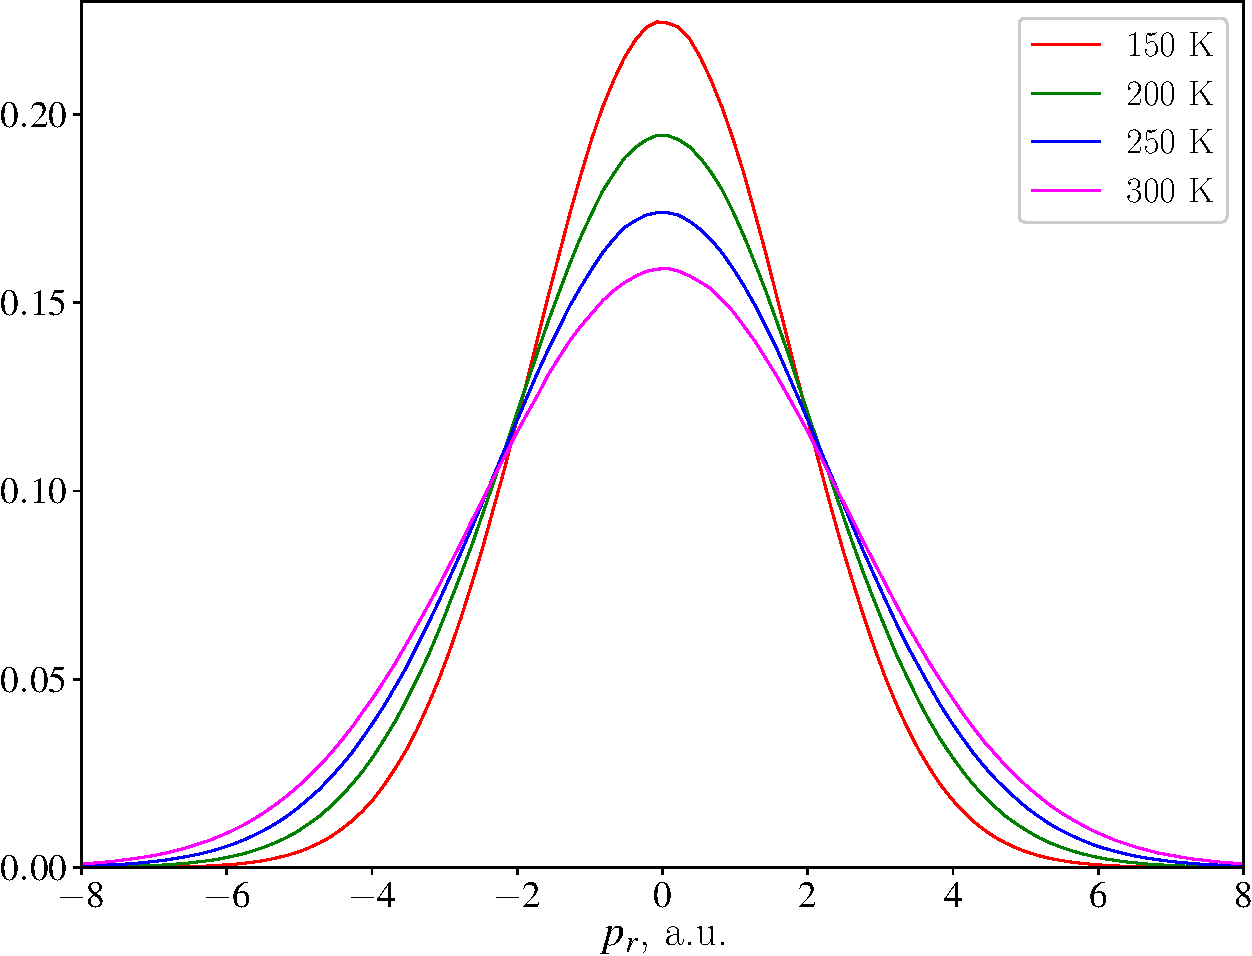
\includegraphics[width=0.75\linewidth]{./pictures/two_atom_distributions/pR-crop.pdf} \\
    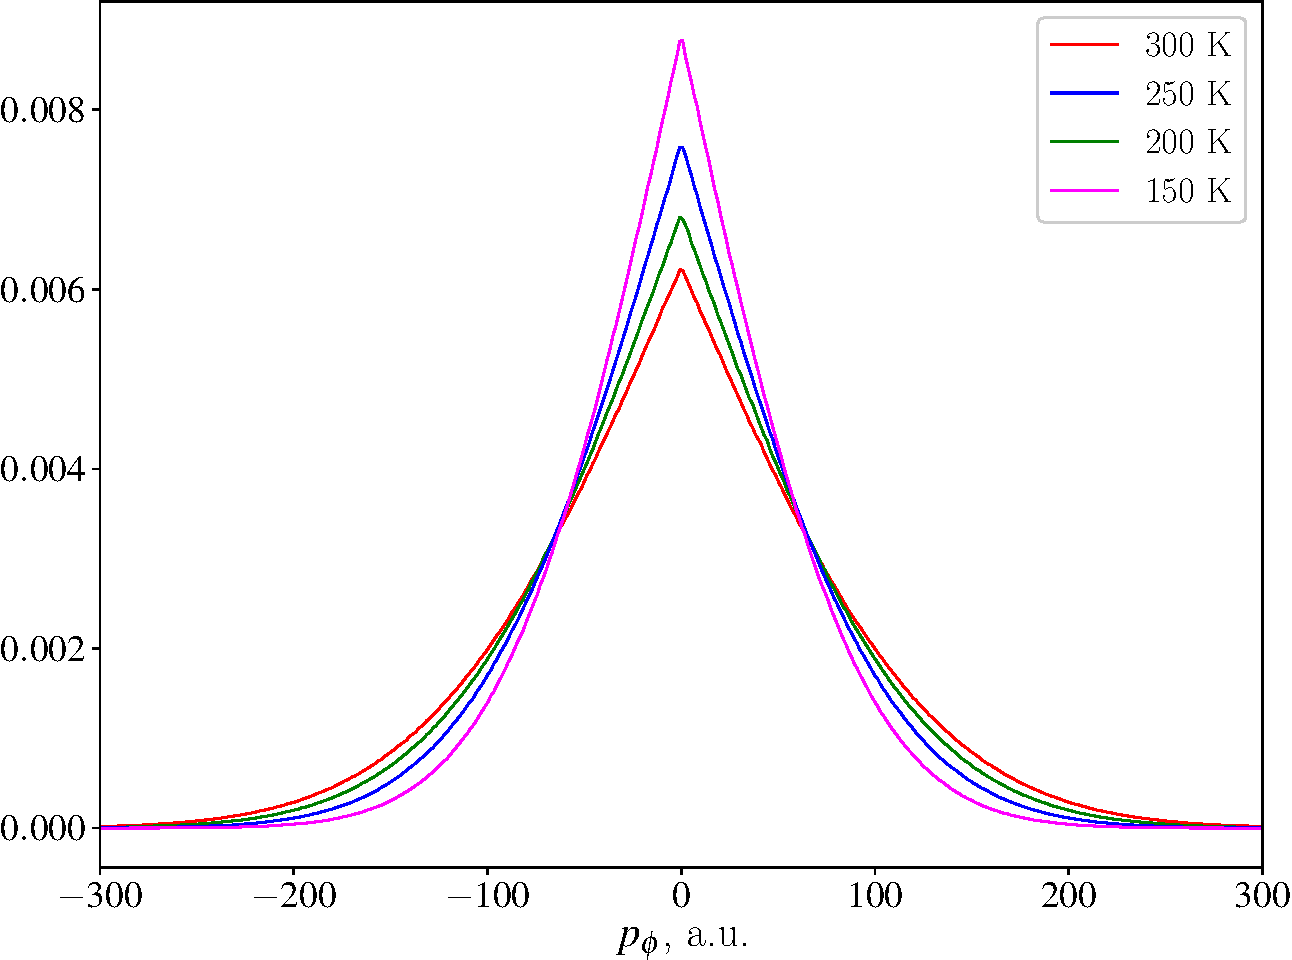
\includegraphics[width=0.75\linewidth]{./pictures/two_atom_distributions/pPhi-crop.pdf}
    \caption{Плотности распределений импульсов $p_r$ и $p_\varphi$ при температурах от 150K до 300K с шагом 50K для системы He$-$Ar. Максимумы плотностей распределений убывают с увеличением температуры. Межатомное расстояние $r_\text{fixed}$ взято равным $40 a_0$. Количество сгенерированых точек при каждой температуре -- $N = 5 \cdot 10^7$.}
\end{figure}

Если переходить теперь к переменным системы координат III, то легко заметить, что плотность распределения импульса $p_r$ совпадает с той, что была получена в системе координат II. Угол $\psi$ не входит в гамильтониан, следовательно распределен с равномерной плотностью. Т.к. якобиан замены декартовых координат и импульсов на координаты и импульсы системы III равен $p_\psi \sin \Theta$ (соотношение, следовательно распределен с равномерной плотностью. Т.к. якобиан замены декартовых координат и импульсов на координаты и импульсы системы III равен $p_\psi \sin \Theta$ (соотношение \eqref{two-atom-planar-jacobian}), то получаем, что плотность распределения импульса $p_\psi$ пропорциональна
\begin{gather}
    \rho(p_\psi) \propto p_\psi \exp \lb -\frac{p_\psi^2}{2 \mu r_\text{fixed}^2 \kb T} \rb, \label{two-atom-ppsi-distribution}
\end{gather}
где константа пропорциональна устанавливается из условия нормировки, оказывается равной $1/(\mu r_\text{fixed}^2 \kb T)$. Из того же якобиана замечаем, что угол $\Theta$ распределен равномерно с косинусом. \par
Распределение для импульса $p_\psi$ может быть установлено и из других соображений. Как уже отмечалось, $p_\psi$ имеет физический смысл модуля углового момента $\mf{J}$. Исходя из выражения \eqref{two-atom-angular-momenta-spherical} получаем, что квадрат модуля углового момента $J^2$ связан с импульсами $p_\varphi$, $p_\theta$ соотношением
\begin{gather}
    J^2 = p_\psi^2 = p_\theta^2 + \frac{p_\varphi^2}{\sin^2 \theta}. \label{two-atom-angular-momenta-connection} 
\end{gather}
Мы уже установили, что слагаемых в правой части \eqref{two-atom-angular-momenta-connection} распределены согласно нормальному распределению. Квадраты нормально распределенных случайных величин распределены согласно хи-квадрат распределению с одной степенью свободы $\chi_1^2$ \cite{castaneda}. А сумма двух одномерных хи-квадрат распределений $\chi_1^2$ дает двумерное хи-квадрат распределение $\chi_2^2$. Наконец, для того, чтобы получить распределение величины $p_\psi$, извлекаем корень из двумерного хи-квадрат распределения $\chi_2^2$ и получаем двумерное хи-распределение $\chi_2$, известное как распределение Рэлея, плотность которого задается  
\begin{gather}
    \rho(x; \sigma) = \frac{x}{\sigma^2} \exp \lb -\frac{x^2}{2 \sigma^2} \rb. \label{rayleigh-density}
\end{gather}

Выражение \eqref{two-atom-ppsi-distribution} является частным случаем \eqref{rayleigh-density} с $\sigma^2 = \mu r_\text{fixed}^2 \kb T$.

\begin{figure}[H]
    \centering
    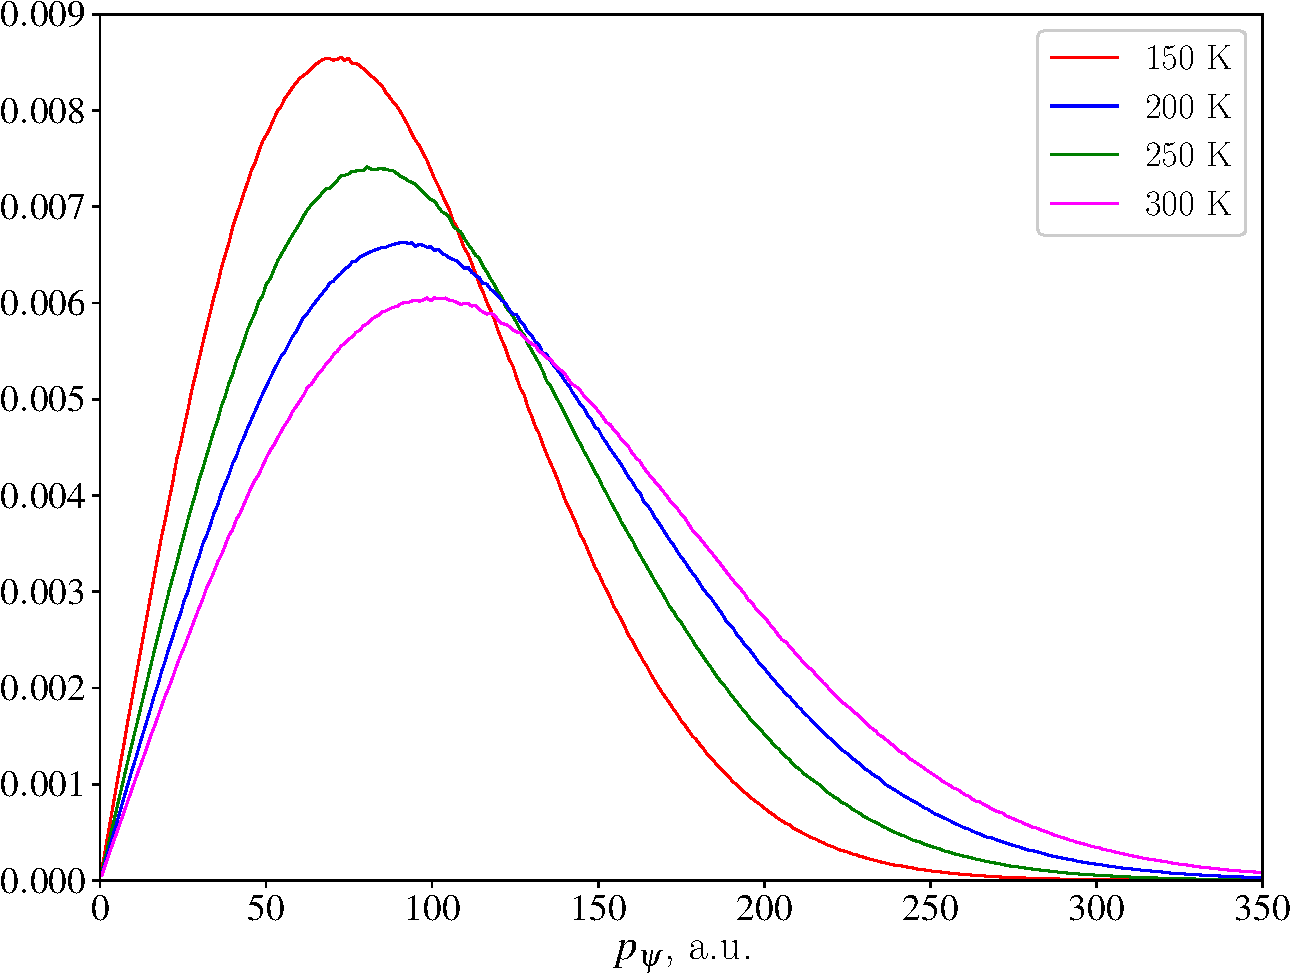
\includegraphics[width=0.75\linewidth]{./pictures/two_atom_distributions/pPsi-crop.pdf}
    \caption{Плотности распределений импульса $p_\psi$ при температурах от 150К до 300К с шагом 50К для системы He$-$Ar. Максимумы распределений уменьшаются и сдвигаются вправо с уменьшением температуры. Межатомное расстояние $r_\text{fixed}$ было взято равным $40a_0$. Количество сгенерированных точек при каждой температуре -- $N = 5 \cdot 10^7$.}
\end{figure}

\section{Спектральная функция при рассмотрении динамики столкновения в плоскости} \label{section:spectral_function_in_plane}

Рассмотрим спектральную функцию,связанную с функцией автокорреляции суммарного дипольного момента преобразованием Фурье
\begin{gather}
    J(\omega) = \intty \mean{ \bs{\mu}(0) \bs{\mu}(t) } e^{-i \omega t} dt.
\end{gather}

Мы будем пользоваться приближением бинарных столкновений, то есть, будем предполагать, что суммарная автокорреляционная функция распадается на сумму автокорреляционных функций индуцированных диполей пар. Для индуцированного дипольного момента пары, для простоты, мы сохраним обозначение $\bs{\mu}$. Итак, мы будем работать со следующим выражением для спектральной функции с трактовкой интеграла как интеграла по начальным условиям классических динамических траекторий, как обсуждалось в пункте \ref{section:correlation_functions} 
\begin{gather}
    J(\omega) = \intty \frac{\displaystyle \idotsint \bs{\mu}(0) \bs{\mu}(t) \, \exp \lb -\frac{\mH}{kT} \rb d\mf{q} \, d\mf{p}}{\displaystyle \idotsint \exp \lb -\frac{\mH}{kT} \rb d\mf{q} \, d\mf{p}} e^{-i \omega t} dt. \label{two-atom-spectral-function1}
\end{gather}

Вектор координат при рассмотрении в плоскости столкновений равен $\mf{q} = \lc r, \psi, \Phi, \Theta \rc$, а вектор импульсов -- $\mf{p} = \lc p_r, p_\psi \rc$. Кроме того, согласно пункту \ref{section:averaging} в интеграле появляется дополнительный весовой множитель, равный $\text{Jac} = p_\psi \sin \Theta$. Следовательно, полное интегральное выражение в этой системе координат выглядит следующим образом
\begin{gather}
    J(\omega) = \intty e^{-i\omega t} dt \frac{\displaystyle \int\limits_0^\infty dr \intty dp_r \int\limits_0^{2\pi} d\psi \int\limits_0^\infty p_\psi dp_\psi \int\limits_0^\pi \sin \Theta d\Theta \int\limits_0^{2\pi} d\Phi \bs{\mu}(0) \bs{\mu}(t) \exp \lb -\frac{\mH}{kT} \rb}{\displaystyle \int\limits_0^\infty dr \intty dp_r \int\limits_0^{2\pi} d\psi \int\limits_0^\infty p_\psi dp_\psi \int\limits_0^\pi \sin \Theta d\Theta \int\limits_0^{2\pi} d\Phi \exp \lb -\frac{\mH}{kT} \rb}. \label{two-atom-spectral-function2}
\end{gather}

Заметим, что ни дипольный момент $\bs{\mu}(t)$, ни гамильтониан $\mH$ не зависят от углов $\Phi$, $\Theta$. Проинтегрировав по ним, мы получаем фактор $4 \pi$ как в числителе, так и знаменателе, поэтому суммарно никаких дополнительных множителей не возникает.
\begin{gather}
    J(\omega) = \intty e^{-i\omega t} dt \frac{\displaystyle \int\limits_0^\infty dr \intty dp_r \int\limits_0^{2\pi} d\psi \int\limits_0^\infty p_\psi dp_\psi \bs{\mu}(0) \bs{\mu}(t) \exp \lb -\frac{\mH}{kT} \rb}{\displaystyle \int\limits_0^\infty dr \intty dp_r \int\limits_0^{2\pi} d\psi \int\limits_0^\infty p_\psi dp_\psi \exp \lb -\frac{\mH}{kT} \rb}. \label{two-atom-spectral-function3}
\end{gather}

Как известно, решение задачи о движении частицы с приведенной массой $\mu$ в центральном поле можно получить, основываясь на законах сохранения энергии и углового момента в интегральном виде \cite{landau-volume1}. Гамильтониан, записанный в полярных координатах, определенных в плоскости движения (система III), 
\begin{gather}
    \mH_\text{plane} = \frac{p_r^2}{2\mu} + \frac{p_\psi^2}{2\mu r^2} + U(r) = E,
\end{gather}
%
является интегралом движения. Как уже отмечалось, импульс $p_\psi$ имеет смысл модуля вектора углового момента, следовательно, также является интегралом движения. Решение уравнений движений в интегральном виде выглядит следующим образом \cite{landau-volume1} 
\begin{gather}
    t = \int\limits_{r_\text{нач}}^{r} \frac{dr}{\displaystyle \sqrt{\frac{2}{\mu} \lb E - U(r) \rb - \frac{p_\psi^2}{\mu^2 r^2}}}, \label{two-atom-change1} \\
    \psi = \int\limits_{r_\text{нач}}^{r} \frac{\displaystyle \frac{p_\psi}{r^2} dr}{\displaystyle \sqrt{2\mu \lb E - U(r) \rb - \frac{p_\psi^2}{r^2}}}, \label{two-atom-change2}
\end{gather}
где $r_\text{нач}$ -- начальное значение межатомного расстояния, а $r$ -- межатомное расстояние в момент времени $t$.  

Рассмотрим замену координат в интеграле в числителе \eqref{two-atom-spectral-function3} следующего вида
\begin{gather}
    \lc r, p_r, \psi, p_\psi \rc \rightarrow \lc (\rfixed), \tau, p_r^\prime, \psi^\prime, p_\psi \rc \label{two-atom-change-variables-time}.
\end{gather}

Физический смысл этой замены координат состоит в том, что вместо того, чтобы начинать классическую траекторию с произвольного межатомного расстояния $r$, мы хотим использовать фиксированное начальное расстояние $\rfixed$ ($\rfixed$ взят в скобках, потому что фиксирован для всех траекторий). Переменная $\tau$ задает время, за которое межатомное расстояние становится равным $r$. Если взять исходное $\rfixed$ бесконечно большим, то набор переменных $\lc \tau, p_r^\prime, \psi^\prime, p_\psi \rc$ опишет тот же массив свободно-разлетных траекторий, что и набор переменных $\lc r, p_r, \psi, p_\psi \rc$. Понятно, что в интеграле \eqref{two-atom-spectral-function3} нам нужно перечислить лишь те классические траектории, на которых межатомное расстояние уменьшилось до такой степени, чтобы появился значительный индуцированный дипольный момент. Поэтому, если мы положим $\rfixed$ больше некоторого расстояния, за которым мы считаем индуцированный дипольный момент равным нулю, то мы перечислим весь значимый массив траекторий (классические траектории, минимальное сближение между атомами в ходе которых больше $\rfixed$, не будут тогда учтены в интеграле, но и вклад от них равен нулю). Подходящее расстояние $\rfixed$ следует подбирать на основании радиальной зависимости индуцированного дипольного момента для каждой конкретной системы по-своему. Отметим, что импульс $p_\psi$ является интегралом движения, поэтому он сохраняется при описанной замене. \par
Для оговоренного набора траекторий замена переменных \eqref{two-atom-change-variables-time} является взаимоднозначной в силу единственности решения системы дифференциальных уравнений с начальными условиями Коши. \par
Заметим, что интегральные выражения \eqref{two-atom-change1}, \eqref{two-atom-change2} описывают ровно половину классической траектории -- от $\rfixed$ до поворотной точки $r_0$, определяемой уравнением
\begin{gather}
    \frac{2}{\mu} \lb E - V(r_0) - \frac{p_\psi^2}{2 \mu r_0^2} \rb = 0.
\end{gather}
Классические траектории столкновения двух тел являются симметричными относительно поворотной точки \cite{goldstein}, поэтому мы без ограничения общности можем рассматривать только ту половину траектории, в ходе которой происходит разлет двух тел от поворотной точки $r_0$ до некоторого выбранного значения $\rfixed$. Другими словами, будем рассматривать такие наборы начальных условий $\lc r, p_r, \psi, p_\psi \rc$,  в которых импульсы $p_r$ являются положительными и будем сопоставлять им наборы начальных условий $\lc \tau, p_r^\prime, \psi^\prime, p_\psi \rc$, в которых импульсы $p_r^\prime$ также являются положительными величинами. \par
Итак, координаты $\tau$, $p_r^\prime$, $\psi^\prime$ связаны с исходными $r$, $p_r$, $\psi$ следующими соотношениями
\begin{gather}
    \lc
    \begin{aligned}
        \tau &= \int\limits_r^{\rfixed} \frac{dr^\prime}{\displaystyle \sqrt{\frac{2}{\mu} \lb E - U(r^\prime) - \frac{p_\psi^2}{2 \mu r^{\prime 2}} \rb}}, \\
        \psi^\prime &= \psi + \int\limits_r^{\rfixed} \frac{\displaystyle \frac{p_\psi}{r^{\prime 2}} dr^\prime}{\displaystyle \sqrt{2\mu \lb E - U(r^\prime) - \frac{p_\psi^2}{2 \mu r^{\prime 2}} \rb}}, \\
        p_r^\prime &= \sqrt{2 \mu \lb E - \frac{p_\psi^2}{2 \mu \rfixed^2} - U(\rfixed) \rb},
    \end{aligned}
    \right. \label{two-atom-change3}
\end{gather}
%
где последнее соотношение получено исходя из закона сохранении энергии в форме
\begin{gather}
    E = \frac{p_r^2}{2\mu} + \frac{p_\psi^2}{2 \mu r^2} + U(r) = \frac{p_r^{\prime 2}}{2 \mu} + \frac{p_\psi^2}{2 \mu \rfixed^2} + U(\rfixed). 
\end{gather}

Учитывая в какой форме записаны соотношения \eqref{two-atom-change3}, найдем якобиан $\displaystyle \Bigg\vert \frac{\partial \lsq \tau, p_r^\prime, \psi^\prime, p_\psi \rsq}{\partial \lsq r, p_r, \psi, p_\psi \rsq} \Bigg \vert$, а затем, пользуясь тем, что якобианы обратны друг к другу
\begin{gather}
    \Bigg\vert \frac{\partial \lsq \tau, p_r^\prime, \psi^\prime, p_\psi \rsq}{\partial \lsq r, p_r, \psi, p_\psi \rsq} \Bigg \vert \cdot \Bigg\vert \frac{\partial \lsq r, p_r, \psi, p_\psi \rsq}{\partial \lsq \tau, p_r^\prime, \psi^\prime, p_\psi \rsq} \Bigg \vert = 1,
\end{gather}
%
найдем интересующий нас якобиан
\begin{gather}
    \text{Jac} = \Bigg\vert \frac{\partial \lsq r, p_r, \psi, p_\psi \rsq}{ \partial \lsq \tau, p_r^\prime, \psi^\prime, p_\psi \rsq} \Bigg\vert.
\end{gather}

Итак, матрица якобиана $\text{Jac}^{-1}$ имеет следующую структуру
\begin{gather}
    \text{Jac}^{-1} = 
    \begin{bdmatrix}
        \frac{\partial \tau}{\partial r} & \frac{\partial \tau}{\partial p_r} & \frac{\partial \tau}{\partial \psi} & \frac{\partial p_\psi}{\partial r} \\
        \frac{\partial p_r^\prime}{\partial r} & \frac{\partial p_r^\prime}{\partial p_r} & \frac{\partial p_r^\prime}{\partial \psi} & \frac{\partial p_r^\prime}{\partial p_\psi} \\
        \frac{\partial \psi^\prime}{\partial r} & \frac{\partial \psi^\prime}{\partial p_r} & \frac{\partial \psi^\prime}{\partial \psi} & \frac{\partial \psi^\prime}{\partial p_\psi} \\
        \frac{\partial p_\psi}{\partial r} & \frac{\partial p_\psi}{\partial p_r} & \frac{\partial p_\psi}{\partial \psi} & \frac{\partial p_\psi}{\partial p_\psi} 
    \end{bdmatrix} = 
    \begin{bdmatrix}
        a & b & 0 & c \\
        d & e & 0 & f \\
        g & h & 1 & k \\
        0 & 0 & 0 & 1
    \end{bdmatrix}.
\end{gather}

Все производные по $\psi$, за исключением $\partial \psi^\prime / \partial \psi$, равны 0, т.к. $\psi$ не входит в выражениях для соответствующих переменных. Производная же $\partial \psi^\prime / \partial \psi$ равна 1, потому что $\psi$ только аддитивно входит в выражение для $\psi^\prime$.
Переменная $p_\psi$ остается неизменной в результате замены, поэтому последняя строчка матрицы оказывается такой простой. \par
Вследствие особенностей структуры матрицы, получается, что детерминант матрицы якобиана $\text{Jac}^{-1}$ зависит только от 4 элементов
\begin{gather}
    \det \lc \text{Jac}^{-1} \rc = a \cdot e - b \cdot d.  
\end{gather}

Явные выражения для этих элементов матрицы выглядят следующим образом 
\begin{gather}
    a = \frac{\partial \tau}{\partial r} = -\frac{\mu}{p_r} - \frac{1}{\mu} \lb \frac{dU}{dr} - \frac{p_\psi^2}{\mu r^3} \rb \cdot I_1, \\ 
    b = \frac{\partial \tau}{\partial p_r} = - \frac{p_r}{\mu^2} I_1, \\ 
    d = \frac{\partial p_r^\prime}{\partial r} = \frac{\displaystyle \mu \lb \frac{dU}{dr} - \frac{p_\psi^2}{\mu r^3} \rb}{\displaystyle \sqrt{2\mu \lb E - \frac{p_\psi^2}{2 \mu \rfixed^2} - U(\rfixed) \rb}} = \frac{\mu}{p_r^\prime} \lb \frac{dU}{dr} - \frac{p_\psi^2}{\mu r^3} \rb, \\
    e = \frac{\partial p_r^\prime}{\partial p_r} = \frac{p_r}{\displaystyle \sqrt{2\mu \lb E - \frac{p_\psi^2}{2 \mu \rfixed^2} - U(\rfixed) \rb}} = \frac{p_r}{p_r^\prime},
\end{gather}
%
где введено обозначение 
\begin{gather}
    I_1 = \int\limits_r^{\rfixed} \lsq \frac{2}{\mu} \lb E - U(r^\prime) - \frac{p_\psi^2}{2 \mu r^{\prime 2}} \rb \rsq^{-3/2} dr^\prime. 
\end{gather}

Для полноты, представим остальные элементы матрицы якобиана
\begin{gather}
    c = \frac{\partial \tau}{\partial p_\psi} = -\frac{p_\psi}{\mu} \int\limits_r^{\rfixed} \lb \frac{1}{r^2} - \frac{1}{r^{\prime 2}} \rb \lsq \frac{2}{\mu} \lb E - U(r^\prime) - \frac{p_\psi^2}{2 \mu r^{\prime 2}} \rb \rsq^{-3/2} dr^\prime \\
f = \frac{\partial p_r^\prime}{\partial p_\psi} = \frac{\displaystyle p_\psi \lb \frac{1}{r^2} - \frac{1}{\rfixed^2} \rb}{\displaystyle \sqrt{2 \mu \lb E - \frac{p_\psi^2}{2 \mu \rfixed^2} - U(\rfixed) \rb}} = \frac{p_\psi}{p_r^\prime} \lb \frac{1}{r^2} - \frac{1}{\rfixed^2} \rb \\
    g = \frac{\partial \psi^\prime}{\partial r} = -\frac{p_\psi}{p_r r^2} - \mu p_\psi \lb \frac{dU}{dr} - \frac{p_\psi^2}{\mu r^3} \rb I_2, \\ 
    h = \frac{\partial \psi^\prime}{\partial p_r} = -p_\psi p_r \cdot I_2, \\ 
    k = \frac{\partial \psi^\prime}{\partial p_\psi} = \int\limits_r^{\rfixed} \frac{1}{r^{\prime 2}} \lsq 2 \mu \lb E - U(r^\prime) - \frac{p_\psi^2}{2 \mu r^2} \rb \rsq \lsq 2 \mu \lb E - U(r^\prime) - \frac{p_\psi^2}{2 \mu r^{\prime 2}} \rb\rsq^{-3/2} dr^\prime,
\end{gather}
%
где было введено обозначение
\begin{gather}
    I_2 = \int\limits_r^{\rfixed} \frac{dr^\prime}{r^{\prime 2}} \lsq 2 \mu \lb E - U(r^\prime) - \frac{p_\psi^2}{2 \mu r^{\prime 2}} \rb \rsq^{-3/2}.
\end{gather}

Итак, якобианы оказываются равными
\begin{gather}
    \Bigg\vert \frac{\partial \lsq \tau, p_r^\prime, \psi^\prime, p_\psi \rsq}{\partial \lsq r, p_r, \psi, p_\psi \rsq} \Bigg\vert = \frac{\mu}{p_r^\prime}, \quad \Bigg\vert \frac{\partial \lsq r, p_r, \psi, p_\psi \rsq}{\partial \lsq \tau, p_r^\prime, \psi^\prime, p_\psi \rsq} \Bigg\vert = \frac{p_r^\prime}{\mu}.
\end{gather}

Следовательно, выражение для спектральной функции \eqref{two-atom-spectral-function3} может быть переписано в виде
\begin{gather}
    J(\omega) = \frac{1}{\Gamma_0} \intty e^{-i \omega t} dt \int\limits_0^\infty d\tau \intty \frac{p_r^\prime}{\mu} dp_r^\prime \int\limits_0^{2\pi} d\psi^\prime \int\limits_0^\infty p_\psi dp_\psi \bs{\mu}(0) \bs{\mu}(\tau) \exp \lb -\frac{\mH_\text{plane}}{kT} \rb,
\end{gather}
%
где через $\Gamma_0$ обозначен интеграл, находящийся в знаменателе \eqref{two-atom-spectral-function3}
\begin{gather}
    \Gamma_0 = \int\limits_0^\infty dr \intty dp_r \int\limits_0^{2\pi} d\psi \int\limits_0^\infty p_\psi dp_\psi \exp \lb -\frac{\mH_\text{plane}}{kT} \rb.
\end{gather}

Переставив интеграл по времени $t$ c интегралами по переменным $\tau$, $p_r^\prime$, $\psi^\prime$ и $p_\psi$, воспользуемся корреляционной теоремой \eqref{correlation-theorem}
\begin{gather}
    J(\omega) = \frac{1}{\Gamma_0} \int\limits_0^\infty \frac{p_r^\prime}{\mu} dp_r^\prime \int\limits_0^{2\pi} d\psi^\prime \int\limits_0^\infty p_\psi dp_\psi \Bigg\vert \intty \bs{\mu}(t) e^{i \omega t} dt \Bigg\vert^2 \exp \lb -\frac{\mH_\text{plane}}{k T} \rb. \label{two-atom-spectral-function4}
\end{gather}

\iffalse
Integral ratio:
\begin{gather}
    \int \exp \lb -\frac{T_H}{kT} \rb d \psi d p_r dp_\psi = 2 \pi^2 \mu k T r \\
    \int \exp \lb -\frac{T_H}{kT} \rb dr d\psi dp_r dp_\psi = \pi^2 \mu k T r^2 \\
    \frac{\int \exp \lb -\frac{T_H}{kT} \rb d\psi dp_r dp_\psi}{\int \exp \lb -\frac{T_H}{k T} \rb dr d\psi dp_r dp_\psi} = \frac{2}{r}
\end{gather}
\fi

\section{Трансляционные спектры газовой смеси He$-$Ar}

Экспериментальные исследования газовых смесей инертных газов He$-$Ar и Ne$-$Ar производились в работах \cite{bosomworth1965_part1, bosomworth1965_part2} при околокомнатных температурах. Полученные в более ранней работе \cite{kiss1959} данные ограничены спектральным диапазоном от 350 до 700 см$^{-1}$ и плохо согласуются с более подробными данными, представленными в \cite{bosomworth1965_part2}, поэтому при комнатной температуре сравнение теоретического спектрального профиля мы будем производить с данными из \cite{bosomworth1965_part2}. Трансляционные спектры систем He$-$Ar и Ne$-$Ar при низких температурах экспериментально исследовались в работах \cite{bukhtoyarova1977, bukhtoyarova1977_2, ryzhov1974}. \par 
Исторически при моделировании трансляционных спектров благородных газов авторы пользовались модельными поверхностями потенциальной энергии и дипольного момента. В работе \cite{levine1967} авторы рассматривают прямолинейные классические траектории столкновения в отсутствии межатомного потенциала; в качестве модели функции дипольного момента была взята гауссова функция, которая совершенно не воспроизводит физического поведения дипольного момента, однако позволяет производить аналитические выкладки. Сделанные приближения позволили получить аналитическое выражение для коэффициента поглощения $\alpha(\omega)$ с использованием спецфункций. В результате подгонки параметров функции дипольного момента было получено согласие аналитической модели для коэффициента поглощения с экспериментальными данными. \par
В работе \cite{mcquarrie1968} представлено моделирование столкновительно-индуцированного спектра методом классических траекторий. Авторы использовали потенциал Леннарда-Джонса (6, 12) с параметрами, подогнанными под экспериментальные данные о сечениях рассеяния. Зависимость дипольного момента от расстояния аппроксимировалась экспоненциальной функцией в области малых межатомных расстояний; при больших расстояниях предполагалось, что дипольный момент отсутствует. При помощи подгонки коэффициента, определяющего скорость спада функции дипольного момента от расстояния, авторам удалось добиться неплохого согласия с экспериментальными данными \cite{bosomworth1965_part2}. \par
Работа \cite{sharma1975} посвящена моделированию столкновительно-индуцированного спектра с позиций квантового формализма. Авторы использовали функции дипольного момента, построенные на основе дальнодействующей компоненты с радиальной асимптотикой $r^{-7}$ и короткодействующей компоненты, имеющей экспоненциальный рост с уменьшением расстояния, рассчитанной методом Хартри-Фока. Качество используемых поверхностей потенциальной энергии и дипольного момента не позволило достичь высокого уровня согласия с экспериментальными данными. \par
Работа \cite{meyer1986} Фроммхольда и Мейера является одной из самых ранних работ, в которой была получена \textit{ab initio} повехность дипольного момента и получена на основе нее зависимость спектральной функции $J(\omega)$ в рамках квантового формализма. Расчеты дипольного момента производились методами Хартри-Фока и конфигурационного взаимодействия в разных базисных наборах. Полученные расчетные значениия дипольного момента были аппроксимированы простой аналитической фукнцией. Отклонение спектральной функции от экспериментальных данных не превышает 10\%. \par 
С развитием современных квантовохимических методов поверхности потенциальной энергии и дипольного момента смесей благородных газов были подробно изучены многими авторами \cite{cybulski1999, giece2003, fernandez2004}. Расчеты производились с использованием методов CCSD/CCSD(T) в корреляционно-согласованных базисных наборах, дополненные связевыми функциями, расположенными на равном расстоянии от обоих атомов. В наиболее современной работе\cite{fernandez2004} авторы использовали метод CCSD(T) и базисный набор aug-cc-pV6Z-33211 для расчета поверхности потенциальной энергии и CCSD/d-aug-cc-pVQZ-33211 для расчета поверхности дипольного момента. Для оценки точности поверхности потенциальной энергии авторы рассчитали температурную зависимость смешанного вириального коэффициента $B_{12}(T)$. Авторы отмечают, что полученные ими поверхности находятся в практически полном согласии с даными \cite{cybulski1999}. В наших расчетах мы использовали предложенные авторами аналитические разложения поверхностей потенциальной энергии и дипольного момента. \par
Нашей научной группой в 2014 году была выполнена работа \cite{buryak2014}, в которой было проведено сравнение траекторного и квантового подходов к расчету трансляционных спектров систем He$-$Ar и Ne$-$Ar. При сравнении использовались поверхности потенциальной энергии \cite{fernandez2004}, поверхности дипольного момента \cite{fernandez2004, meyer1986}. Несмотря на то, что квантовые расчеты должны давать более точные спектральные профили, результаты, полученные в траекторном расчете, оказываются в хорошем согласии как с квантовыми расчетами, так и с экспериментальными данными. Было отмечено, что некоторую проблему при классическом моделировании спектра представляет собой процедура десимметризации профиля, которую мы обговорим подробнее позже. \par

\section{Вычислительные аспекты расчета столкновительно$-$ индуцированного спектра методом классических траекторий}

Расчет спектральной функции системы из двух атомов в нашей работе мы будем производить по выражению \eqref{two-atom-spectral-function4}. Вычисление многомерного интеграла будем производить методом Монте-Карло, т.к. при рассмотрении систем с большим количеством вращательных степеней свободы мы сталкнемся с интегралами значительно более высокой размерности, вычисление которых квардратурными методами не представляется возможным. В данном случае при интегрировании квадратурами общие вычислительные затраты могут оказаться меньше, однако т.к. такая схема интегирования оказывается непереносимой на системы, в которых мономеры обладают несколькими вращательными степенями свободы, то мы отказались от ее реализации. Известно, что погрешность метода Монте-Карло асимптотически ведет себя как $N^{-1/2}$, где $N$ -- количество точек, по которым производилась оценка интеграла \cite{sobol}. Такая асимптотика ошибки не позволяет получать очень точных оценок интегралов, что в некоторых задачах оказывается неудовлетворительным. В задаче моделирования континуального спектрального профиля точность порядка $\sim 0.5\%$ оказываеся приемлимой, что достижимо с использованием метода Монте-Карло. Более подробно вопрос о точности получающегося спектрального профиля в нашем подходе мы обсудим после описания вычислительной схемы. \par
Интегрирование в \eqref{two-atom-spectral-function4} мы будем производить методом Монте-Карло с весовой функцией $p_\xi(\bxi) = p_\psi \exp \lb -\mH_\text{plane}(\bxi) / \kb T \rb / \Gamma_1$, где $\bxi = \lc p_R^\prime, \psi^\prime, p_\psi \rc$, а $\Gamma_1$ -- нормировочный множитель, равный
\begin{gather}
    \Gamma_1 = \int\limits_0^\infty dp_r^\prime \intty d\psi^\prime \intty p_\psi \exp \lb -\frac{\mHplane}{\kb T} \rb dp_\psi.
\end{gather}
Выражение \eqref{two-atom-spectral-function4} может быть рассмотрено как математическое ожидание квадрата преобразования Фурье на распределении $\boldsymbol{\xi}$, заданном весовой функции
\begin{gather}
    J(\omega) = \frac{\Gamma_1}{\Gamma_0} \sum_{k = 1}^{\infty} \frac{p_r^\prime(\bxi_k)}{\mu} \Big\vert \intty \bs{\mu}(t; \bxi_k) e^{i \omega t} dt \Big\vert^2, \label{two-atom-spectral-function-mc}
\end{gather}
%
где обозначение $p_r^\prime(\bxi_k)$ подразумевает, что импульс, сопряженный радиальной координате, взят из вектора $\bxi$, реализующего распределение с плотностью $p_\xi$. \par
Основываясь на выкладках, сделанных в параграфе \ref{section:averaging}, несложно получить аналитические выражения для интегралов $\Gamma_0, \Gamma_1$
\begin{gather}
    \Gamma_0 = \int\limits_0^\infty dr \intty dp_r \int\limits_0^{2\pi} d\psi \int\limits_0^\infty p_\psi \exp \lb -\frac{\mHplane}{\kb T} \rb d p_\psi = \frac{4}{3} \pi r_\text{fixed}^3 \lb 2 \pi \mu \kb T \rb^{3/2}, \\
    \Gamma_1 = \int\limits_0^\infty dp_r \int\limits_0^{2\pi} d\psi \int\limits_0^\infty p_\psi \exp \lb -\frac{\mHplane}{\kb T} \rb dp_\psi  = 2 \pi r_\text{fixed}^2 \lb 2 \pi \mu \kb T \rb^{3/2}.
\end{gather}
Таким образом, конечное выражение для спектральной функции, как среднее значение на распределении с плотностью $p_\xi(\bxi)$, приходит к виду
\begin{gather}
    J(\omega) = 2 \pi \rfixed^2 \sum_{k = 1}^\infty \frac{p_r^\prime(\bxi_k)}{\mu} \Big\vert \intty \bs{\mu}(t; \bxi_k) e^{i \omega t} dt \Big\vert^2. \label{two-atom-spectral-function-mc-final}
\end{gather}

Вопрос генерации реализаций случайной величины $\bxi$ с плотностью распределения $p_\xi$ был обсужден в параграфе \ref{section:averaging}. Рассмотрим вопрос расчет классических траекторий рассеяния. Несмотря на то, что для динамических переменных могут быть выписаны квадратурные выражения, которыми мы пользовались в параграфе \ref{section:spectral_function_in_plane}, вычисления по ним производить не очень удобно. В первую очередь неудобство связано с тем, что для вычисления усредняемого выражения в \eqref{two-atom-spectral-function-mc-final} нам потребуется вычислять преобразование Фурье от дипольного момента вдоль траектории, которое эффективно реализуется в виде дискретного преобразования Фурье. Для этого нам потребуются значения дипольного момента $\bs{\mu}(t)$ с равноверным шагом по времени, что вызовет некоторые затруднения при вычисления по квадратурной формуле. Кроме того, квадратуры для всех динамических переменных являются несобственными интегралами, имеющими особенность в поворотной точке. Поэтому траектории рассеяния рассчитывались интегрированием трех уравнений Гамильтона
\begin{gather}
    \lc
    \begin{aligned}
        \dot{r} &= \frac{p_r}{\mu} \\
        \dot{\psi} &= \frac{p_\psi^2}{\mu r^3} - \frac{d U}{d r} \\
        \dot{p_\psi} &= \frac{p_\psi}{\mu r^2}
    \end{aligned}
    \right. \label{two-atom-hamilton-equations}
\end{gather}

Была разработана программа на языке С++, реализующая классический траекторный расчет по описанной схеме. Система уравнений \eqref{two-atom-hamilton-equations} численно интегрировалась при помощи пакета процедур для решения дифференциальных уравнений SUNDIALS \cite{sundials}. Использовались процедуры, реализующие BDF формулы переменного порядка. Решение нелинейных уравнений, возникающих в результате применения BDF формул, происходит с использованием стандартного метода Ньютона. Вычисления производились с двойной точностью со значением параметра, определяющего относительную ошибку решения, равным $10^{-15}$. Так как каждая траектория может быть рассчитана в независимости от остальных, то легко может быть написана программа для расчета массива траекторий в параллельном режиме. В коде была использована библиотека MPI \cite{mpi}, стандартизующая передачу сообщений между узлами параллельного приложения. Приложение реализовано в модели взаимодействия \enquote{ведущий-ведомый}, в которой \enquote{ведущий} процесс отвечает за распределение начальных условий между \enquote{ведомыми} процессами, осуществляющими расчет траекторий. Получив начальное условие, \enquote{ведомый} процесс рассчитывает траекторию рассеяния с внутренним переменным шагом по времени, при этом с фиксированным шагом по времени $\Delta t = 200$ атомных единиц времени (около 5 фс) вдоль траектории вычисляется значение индуцированного дипольного момента и собирается в заранее подготовленный массив, содержащий $L = 2^{15}$ ячеек. Расчет траектории заканчивается в тот момент, когда межатомное расстояние вновь достигает начального значения или количество вычислений дипольного момента превышает $L$. Затем в рамках \enquote{ведомого} процесса осуществляется дискретное преобразование Фурье временной зависимости индуцированного дипольного момента. Выбор длины массива $L$ обусловлен тем, что наиболее эффективно дискретное преобразование Фурье выполняется для массива, длина которого есть некоторая степень двух (так называемое быстрое преобразование Фурье). Согласно выражению \eqref{two-atom-spectral-function-mc-final} вычисляется квадрат преобразования Фурье (трактовка вычисления квадрата обсуждалась в самом начале главы \ref{chapter:two-atom}), умножается на отношение радиального импульса $p_r$ в начальный момент времени к приведенной массе $\mu$ и полученный массив передается на \enquote{ведущий} процесс. \enquote{Ведущий} процесc накапливает результаты \enquote{ведомых} процессов и после усреднения получает спектральную функцию.
    Спектральный профиль, полученный в результате траекторного расчета, представлен на рис. \ref{fig:two-atom-desymmetrizations}.
\begin{figure}
    \centering
    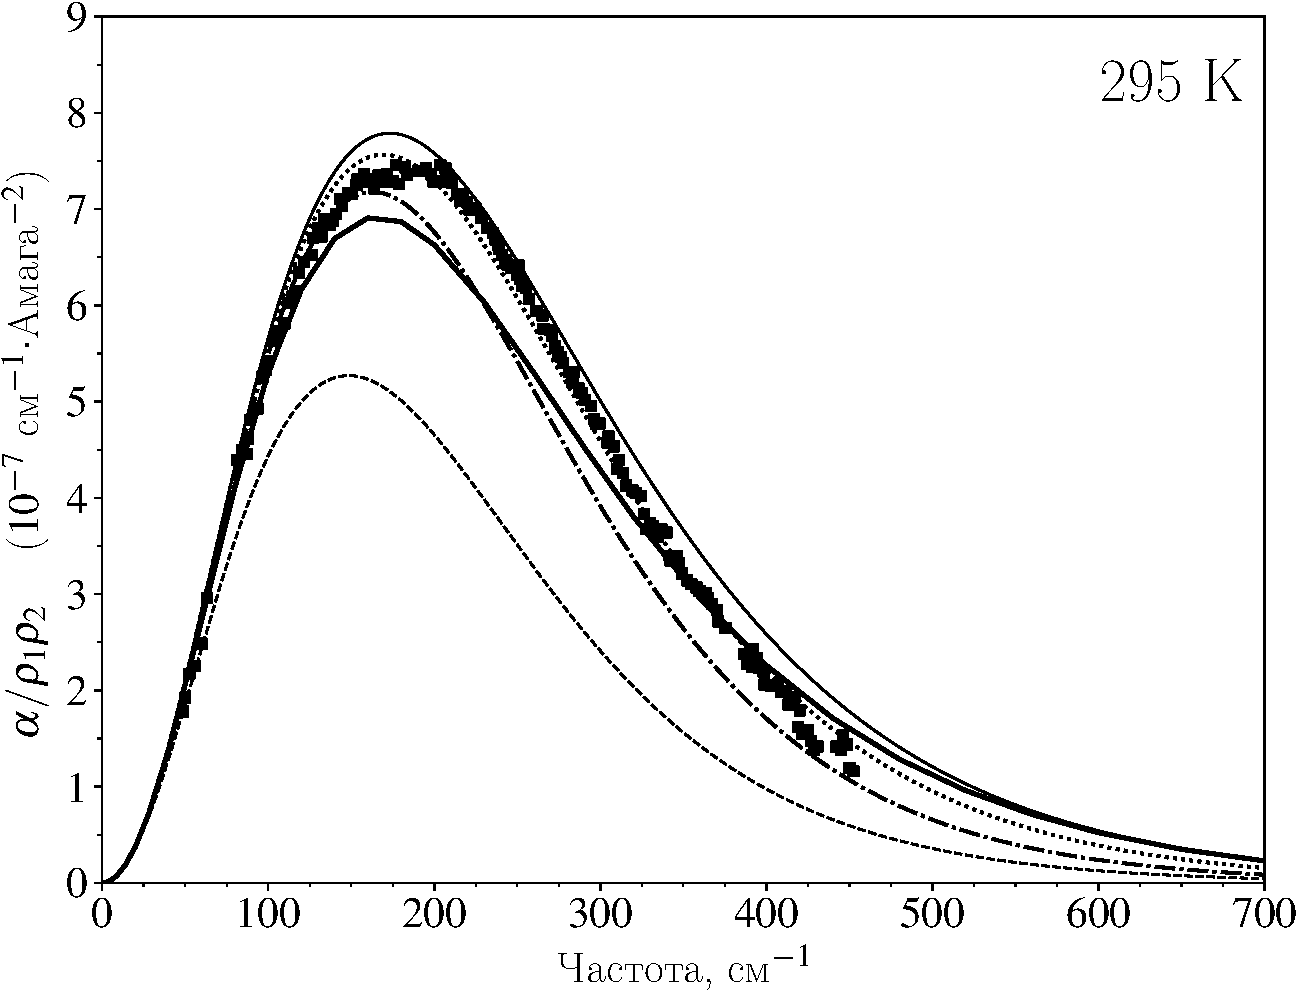
\includegraphics[width=0.7\linewidth]{./pictures/two_atom_spectra/desymmetrizations_295K-crop.pdf}
    \caption{Сравнение классического и квантового спектральных профилей с профилями, полученными в результате применения различных процедур десимметризации. Пунктиром обозначен классический профиль, сплошной толстой линией -- квантовый профиль \cite{buryak2014}, точками с пунктиром -- профиль, полученный в результате применения процедуры D1, точечной линией -- профиль, полученный в результате применения процедуры D2, сплошной линией -- профиль, полученный в результате применения процедуры D3. Квадратами обозначены экспериментальные данные \cite{bosomworth1965_part2}.}
    \label{fig:two-atom-desymmetrizations}
\end{figure}

Как известно, классические траектории обратимы во времени. Это свойство классических траекторий приводит к тому, что автокорреляционная функция дипольного момента $C(t)$ является симметричной функцией от времени \cite{frommhold}
\begin{gather}
    C(t) = C(-t).
\end{gather}

Классическая спектральная функция, получающаяся в результате применения преобразования Фурье к автокорреляционной функции, также оказывается симметричной функции частоты 
\begin{gather}
    J_\text{class.}(\omega) = J_\text{class.}(-\omega). \label{classical-detailed-balance}
\end{gather}

Однако квантовая спектральная функция удовлетворяет так называемому условию детального баланса \cite{frommhold} 
\begin{gather}
    J(-\omega) = J(\omega) \exp \lb -\frac{\hbar \omega}{\kb T} \rb, \label{detailed-balance}
\end{gather}
%
которое может быть получено из выражения \eqref{part1-spectral-function-definition} перестановкой индексов $j, k$. Условие детального баланса \eqref{detailed-balance} отражает разницу в заселенностях исходного и конечного состояний. Ввиду этого, соотношение \eqref{classical-detailed-balance} называют классическим условием детального баланса. \par
Считается, что симметрийная разница между классической и квантовой спектральной функциями может быть устранена при помощи так называемой процедуры десимметризации. Предполагается, что классическую спектральную функцию можно определенным образом \enquotes{десимметризовать} так, что функция, получившаяся в результате, будет удовлетворять квантовому условию детального баланса \cite{borysow1985phenomena}. Однако процедура десимметризации не может быть однозначна задан условием детального баланса -- можно построить бесконечное количество процедур, которые будут приводить к спектральной функции, которая будет удовлетворять квантовому условию детального баланса \cite{frommhold}. Поэтому от процедуры десимметризации дополнительно требуют совпадения десимметрованного классического профиля с квантовым профилем в особенности в области дальних крыльев. \par
В литературе представлен набор различных процедур десимметризации \cite{borysow1985}. Некоторые из них устроены следующим образом:
\begin{gather}
    J_{D1}(\omega) = \frac{2}{1 + \exp \lb -\hbar \omega / \kb T \rb} J_\text{class}(\omega)  \\
    J_{D2}(\omega) = \frac{\hbar \omega}{\kb T} \frac{1}{1 - \exp \lb -\hbar \omega / \kb T \rb} J_\text{class}(\omega) \\
    J_{D3}(\omega) = \exp \lb \frac{\hbar \omega}{2 \kb T} \rb J_\text{class}(\omega)
\end{gather}
В литературе также используется преобразование Эгельстаффа \cite{egelstaff1962}; нами она практически не использовалась, поэтому результаты применения этой процедуры не приводятся. 

\begin{figure}
    \centering
    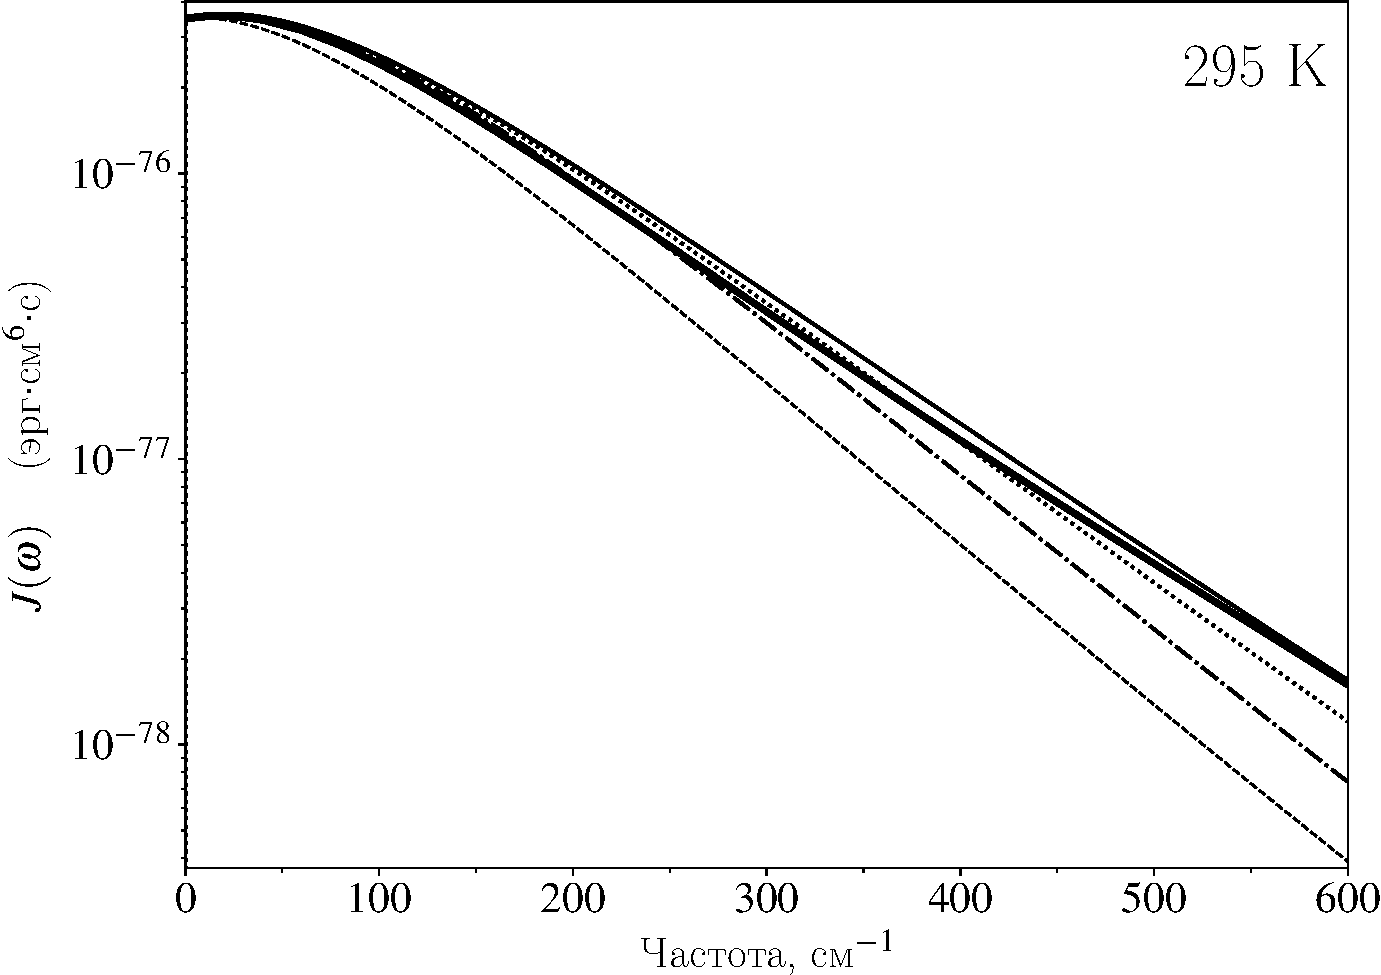
\includegraphics[width=0.7\linewidth]{./pictures/two_atom_spectra/spectral_function_desymmetrizations-crop.pdf}
    \caption{Сравнение крыльев классической, квантовой и десимметризованных спектральных функций системы He$-$Ar при температуре 295 K. Сплошной толстой линией обозначена квантовая спектральная функция \cite{buryak2014}; пунктиром -- классическая спектральная функция; пунктиром с точками -- спектральная функция, полученная в результате процедуры десимметризации D1; точечной линией -- спектральная функция, полученная в результате процедуры десимметризации D2; тонкой сплошной линией -- спектральная функция, полученная в результате процедуры десимметризации D3.}
    \label{fig:desymmetrisation-spectral-functions}
\end{figure}

Несложно убедиться, что приведенные процедуры десимметризации D1-D3 приводят к спектральным функциям, удовлетворяющим квантовому условию детального баланса. Продемонстрируем это на примере десимметризации D3, используя классическое правило детального баланса для $J_\text{class}(\omega)$:
\begin{gather}
    J_{D3}(\omega) = \exp \lb \frac{\hbar \omega}{2 \kb T} \rb J_\text{class}(\omega) \quad \implies \quad J_\text{class}(\omega) = \exp \lb -\frac{\hbar \omega}{2 \kb T} \rb J_{D3}(\omega), \\
    J_{D3}(-\omega) = \exp \lb -\frac{\hbar \omega}{2 \kb T} \rb J_\text{class}(-\omega) = \exp \lb -\frac{\hbar \omega}{2 \kb T} \rb J_\text{class}(\omega), \\
    J_{D3}(-\omega) = \exp \lb -\frac{\hbar \omega}{\kb T} \rb J_\text{D3}(\omega).
\end{gather}

Основываясь на рисунке \ref{fig:desymmetrisation-spectral-functions} замечаем, что при малых частотах все спектральные функции ведут себя примерно примерно одинаковым образом, однако с увеличением частоты различие между ними становится все больше. Одной из наиболее популярной в литературе является процедура D3. Спектральная функция, полученная в результате процедуры D3, переоценивает квантовую спектральную функции в области крыла, однако считается, что около максимума спектра она дает наилучшую оценку. Сравнение при других температурах мы будем производить именно со спектром, полученным в результате процедуры D3. \par
Сравнение с экспериментальными данными на \ref{fig:two-atom-spectra} показывает, что несмотря на проблему выбора подходящей процедуры десимметризации, общее совпадение с экспериментальными данными оказывается неплохим. Отклонения между спектрами, полученными в результате применения различных процедур десимметризации, не превышает отклонения между квантовым профилем и экспериментальными данными.  

\begin{figure}[H]
    \centering
    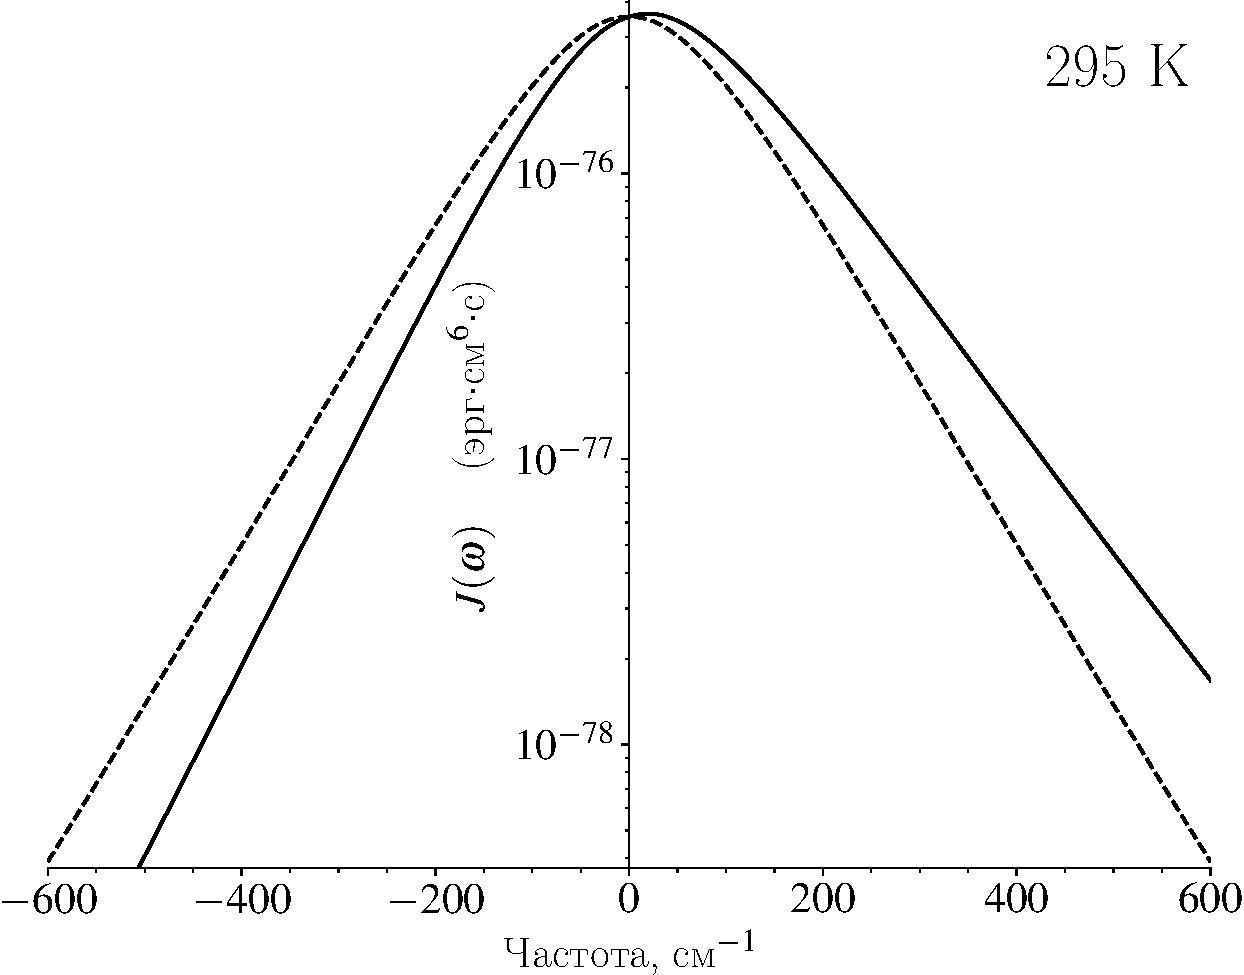
\includegraphics[width=0.49\linewidth]{./pictures/two_atom_spectra/spectral_function_d3-crop.pdf}
    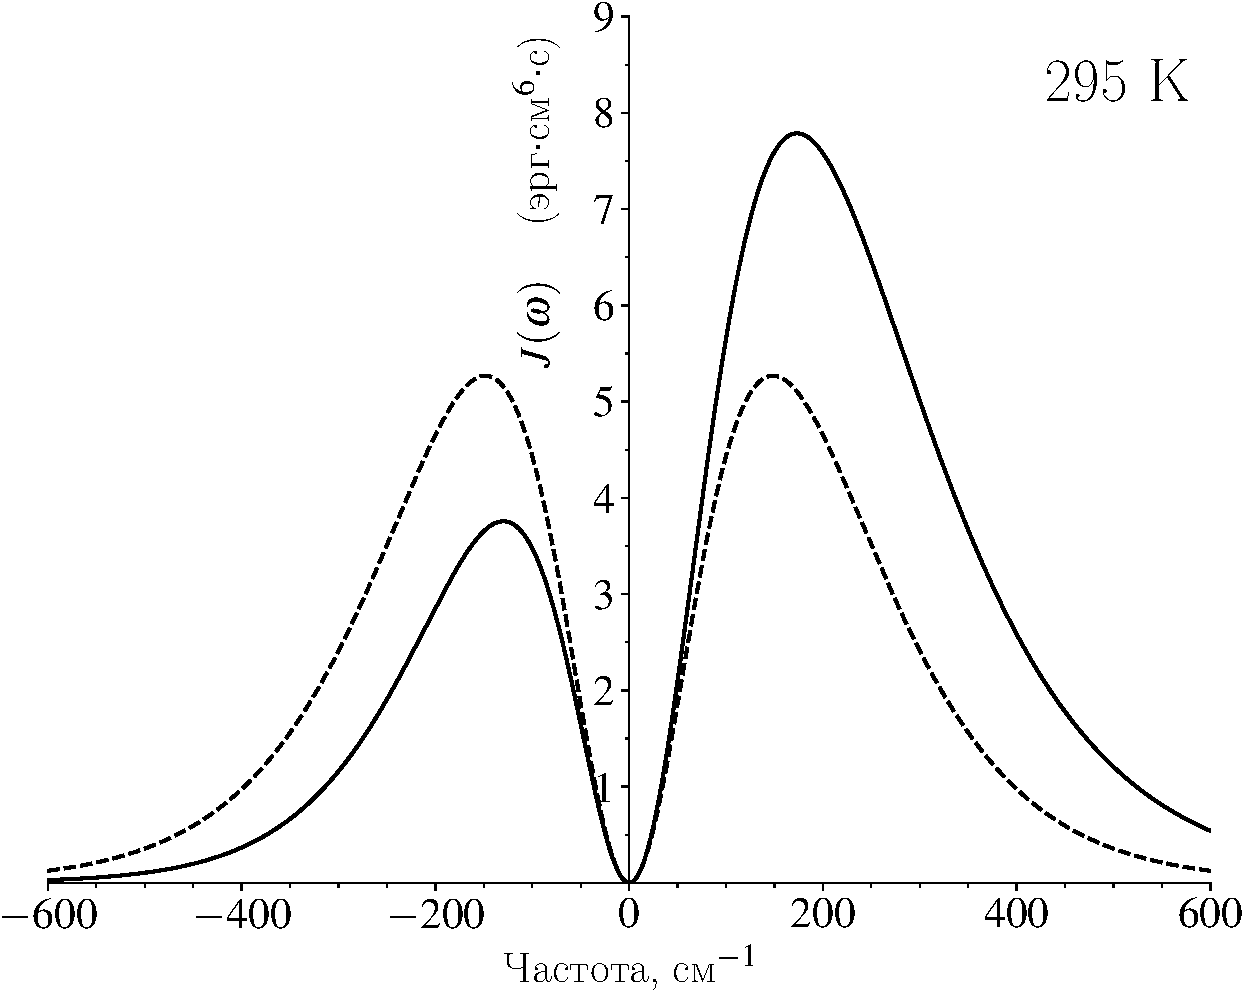
\includegraphics[width=0.49\linewidth]{./pictures/two_atom_spectra/spectrum_effect_d3-crop.pdf}
    \caption{Влияние десимметризации на спектральную функцию и спектральный профиль с учетом отрицательных частот. Пунктиром обозначены классические спектральная функция и профиль; сплошной линией -- полученные из классических в результате процедуры D3.}
\end{figure}


\begin{figure}[H]
    \centering
    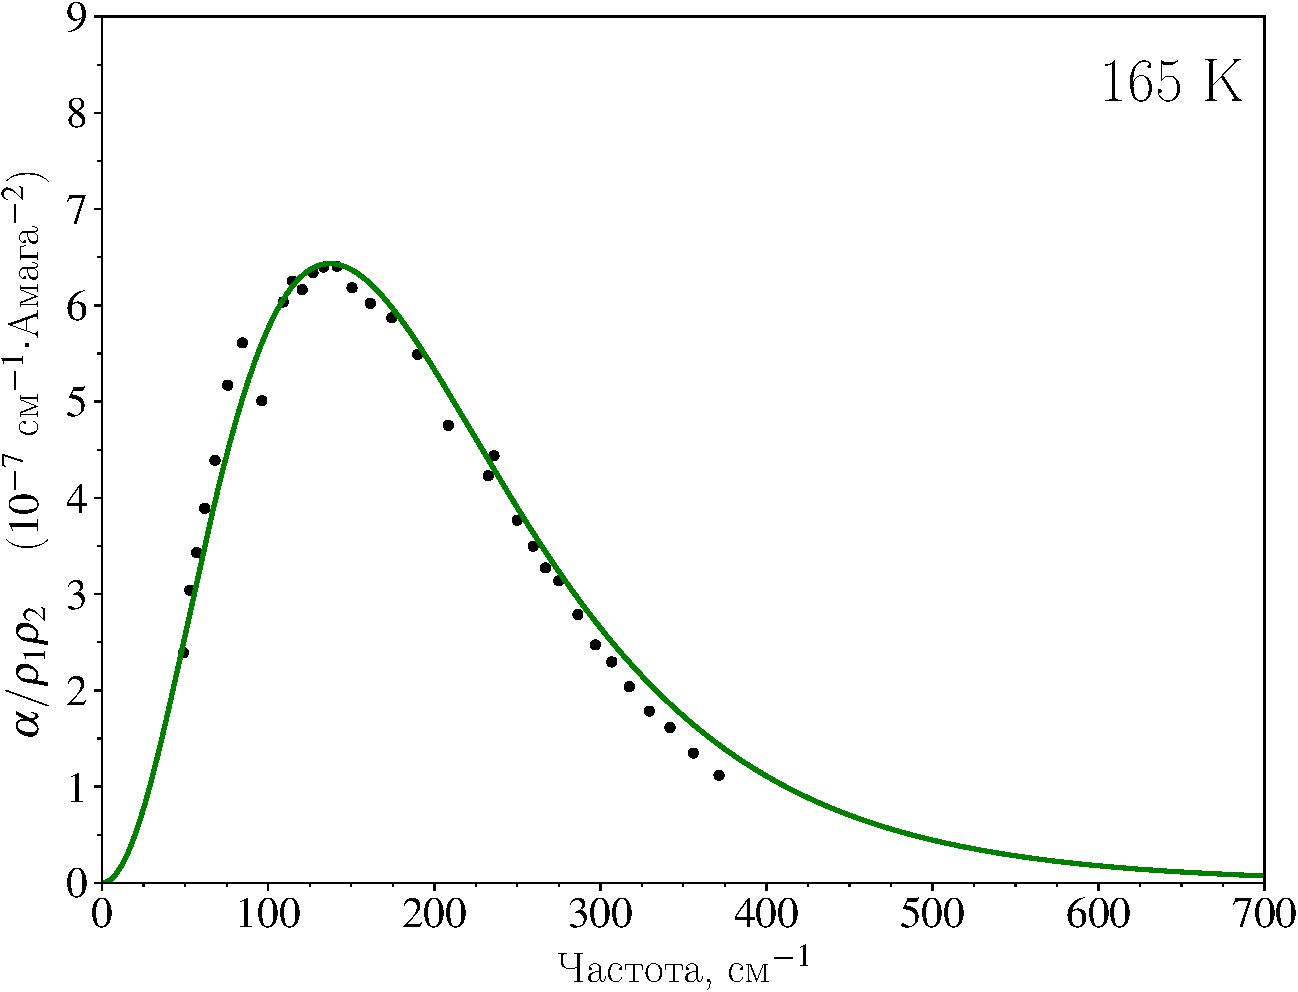
\includegraphics[width=0.49\linewidth]{./pictures/two_atom_spectra/alpha_165K-crop.pdf} 
    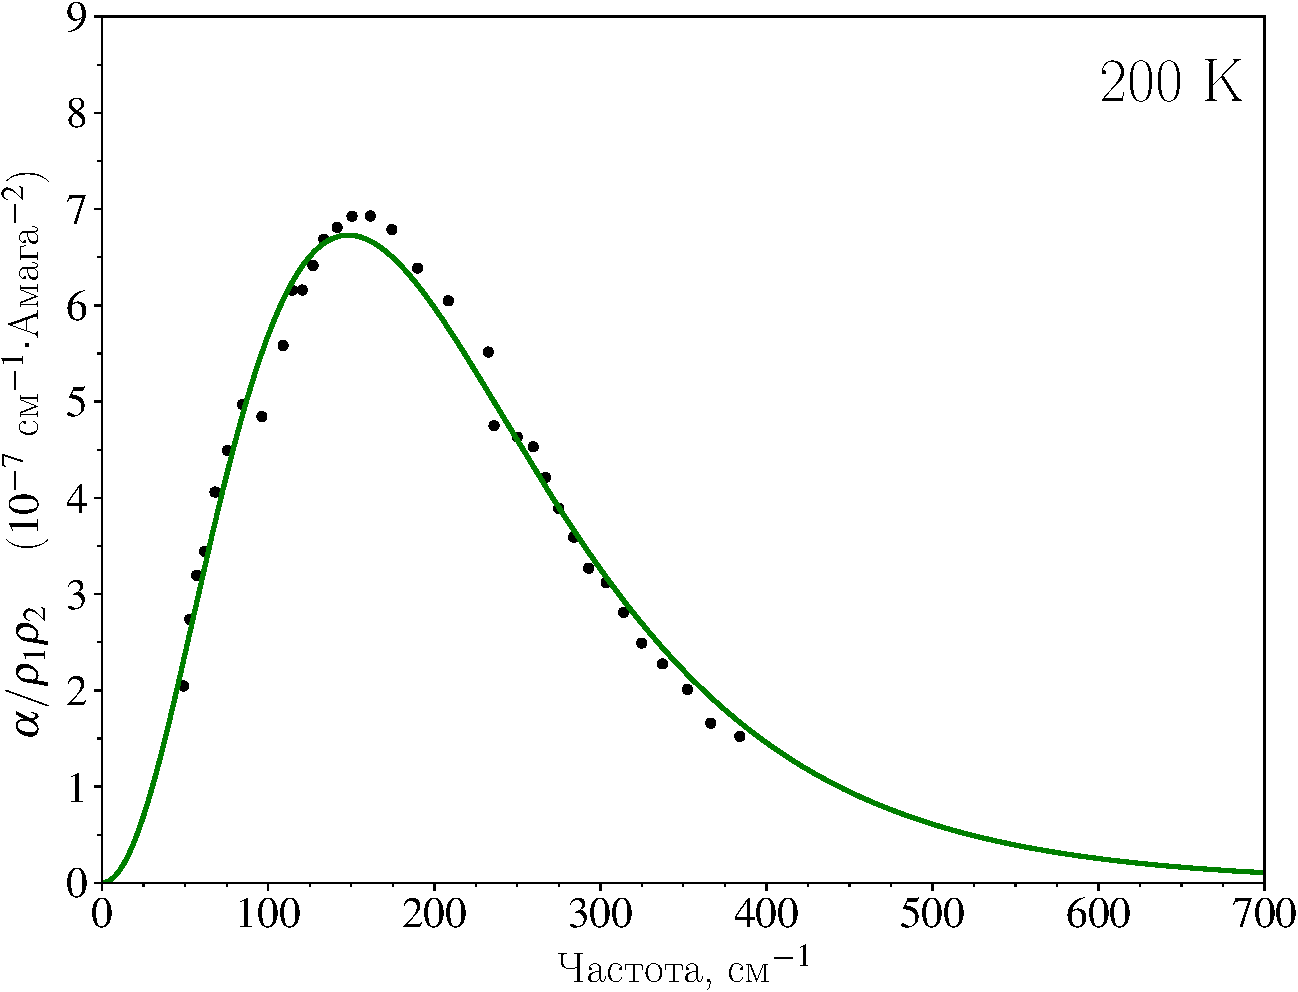
\includegraphics[width=0.49\linewidth]{./pictures/two_atom_spectra/alpha_200K-crop.pdf} \\
    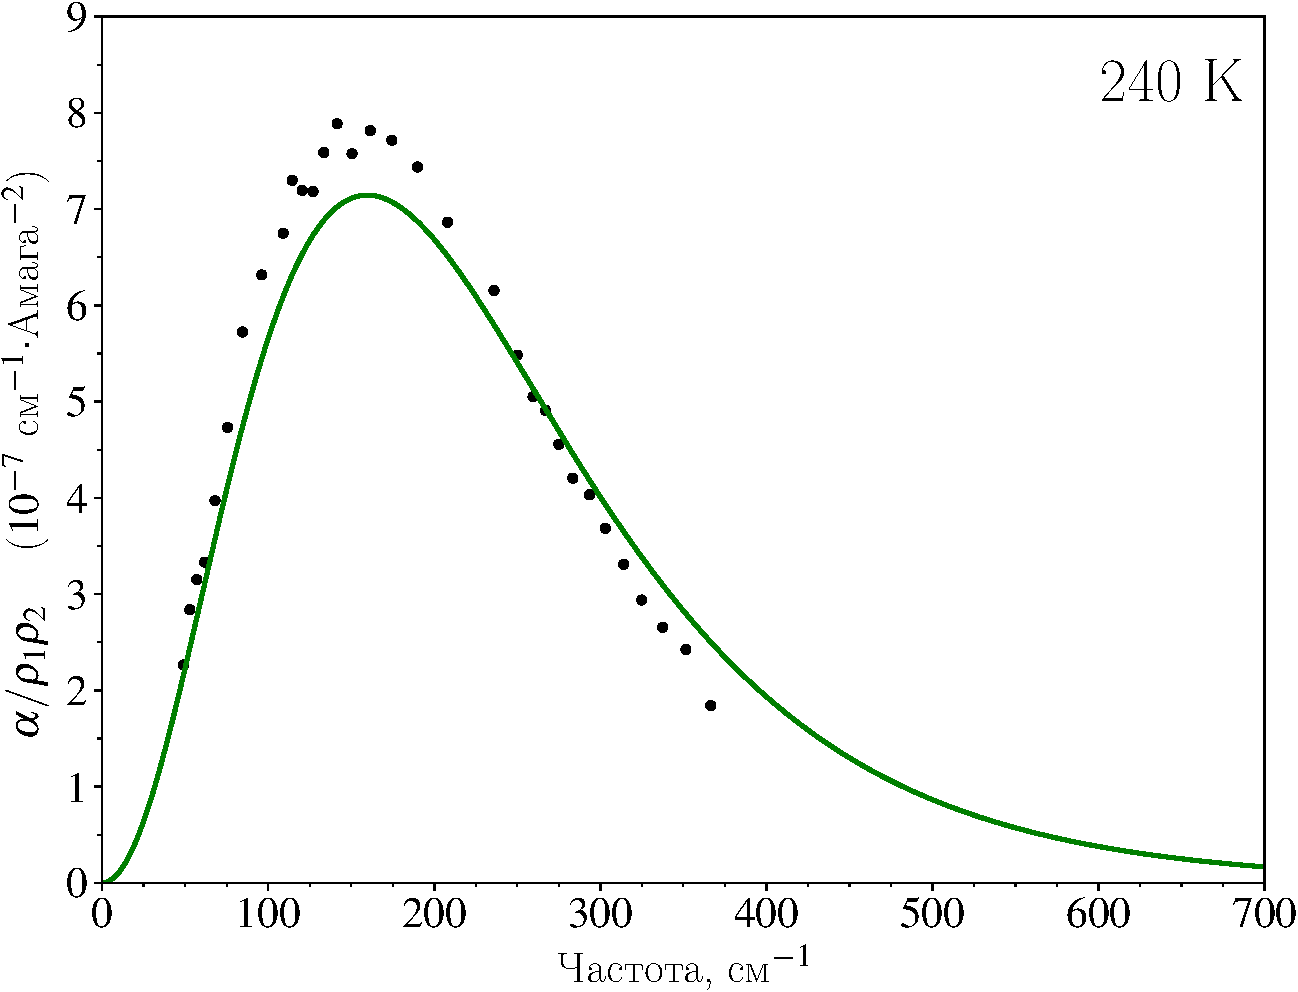
\includegraphics[width=0.49\linewidth]{./pictures/two_atom_spectra/alpha_240K-crop.pdf}
    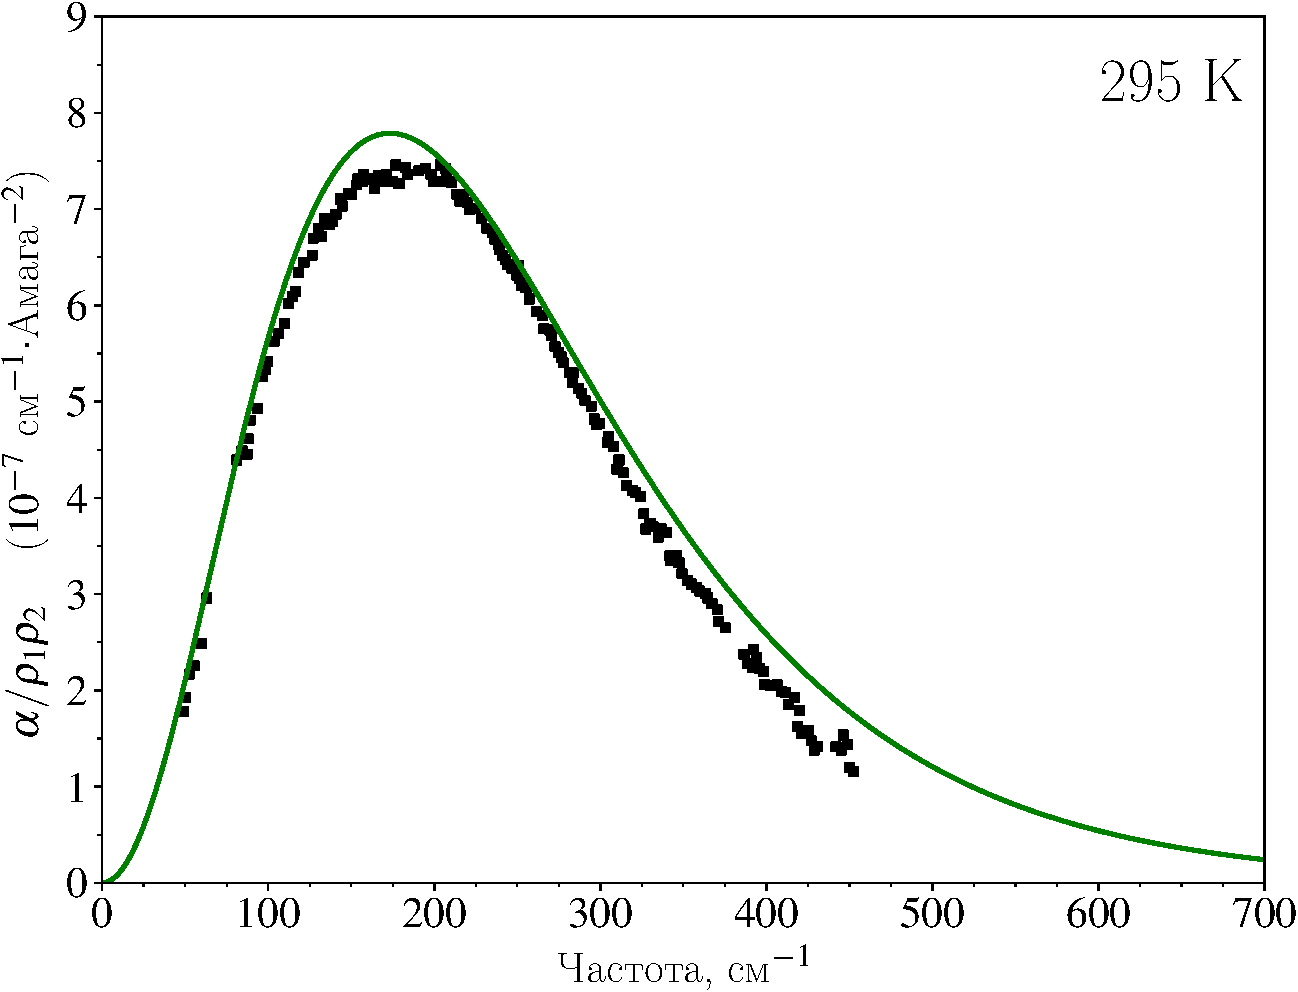
\includegraphics[width=0.49\linewidth]{./pictures/two_atom_spectra/alpha_295K-crop.pdf}
    \caption{Трансляционные спектры системы He$-$Ar при температурах 165K, 200K, 240K и 295K. Черными кружками обозначены экспериментальные данные из \cite{bukhtoyarova1977, bukhtoyarova1977_2, ryzhov1974}, квадратами -- из \cite{bosomworth1965_part2}.}
    \label{fig:two-atom-spectra}
\end{figure}


